%
% $RCSfile: knowledge_schema.tex,v $
%
% Copyright (C) 2002-2008. Christian Heller.
%
% Permission is granted to copy, distribute and/or modify this document
% under the terms of the GNU Free Documentation License, Version 1.1 or
% any later version published by the Free Software Foundation; with no
% Invariant Sections, with no Front-Cover Texts and with no Back-Cover
% Texts. A copy of the license is included in the section entitled
% "GNU Free Documentation License".
%
% http://www.cybop.net
% - Cybernetics Oriented Programming -
%
% http://www.resmedicinae.org
% - Information in Medicine -
%
% Version: $Revision: 1.1 $ $Date: 2008-08-19 20:41:07 $ $Author: christian $
% Authors: Christian Heller <christian.heller@tuxtax.de>
%

\chapter{Knowledge Schema}
\label{knowledge_schema_heading}
\index{Knowledge Schema}

\begin{flushright}
    \textsl{Wise Man's Occupation is Organisation.}\\
    \textsc{Thomas Aquinas}
\end{flushright}

\begin{wrapfigure}[7]{r}{4cm}
    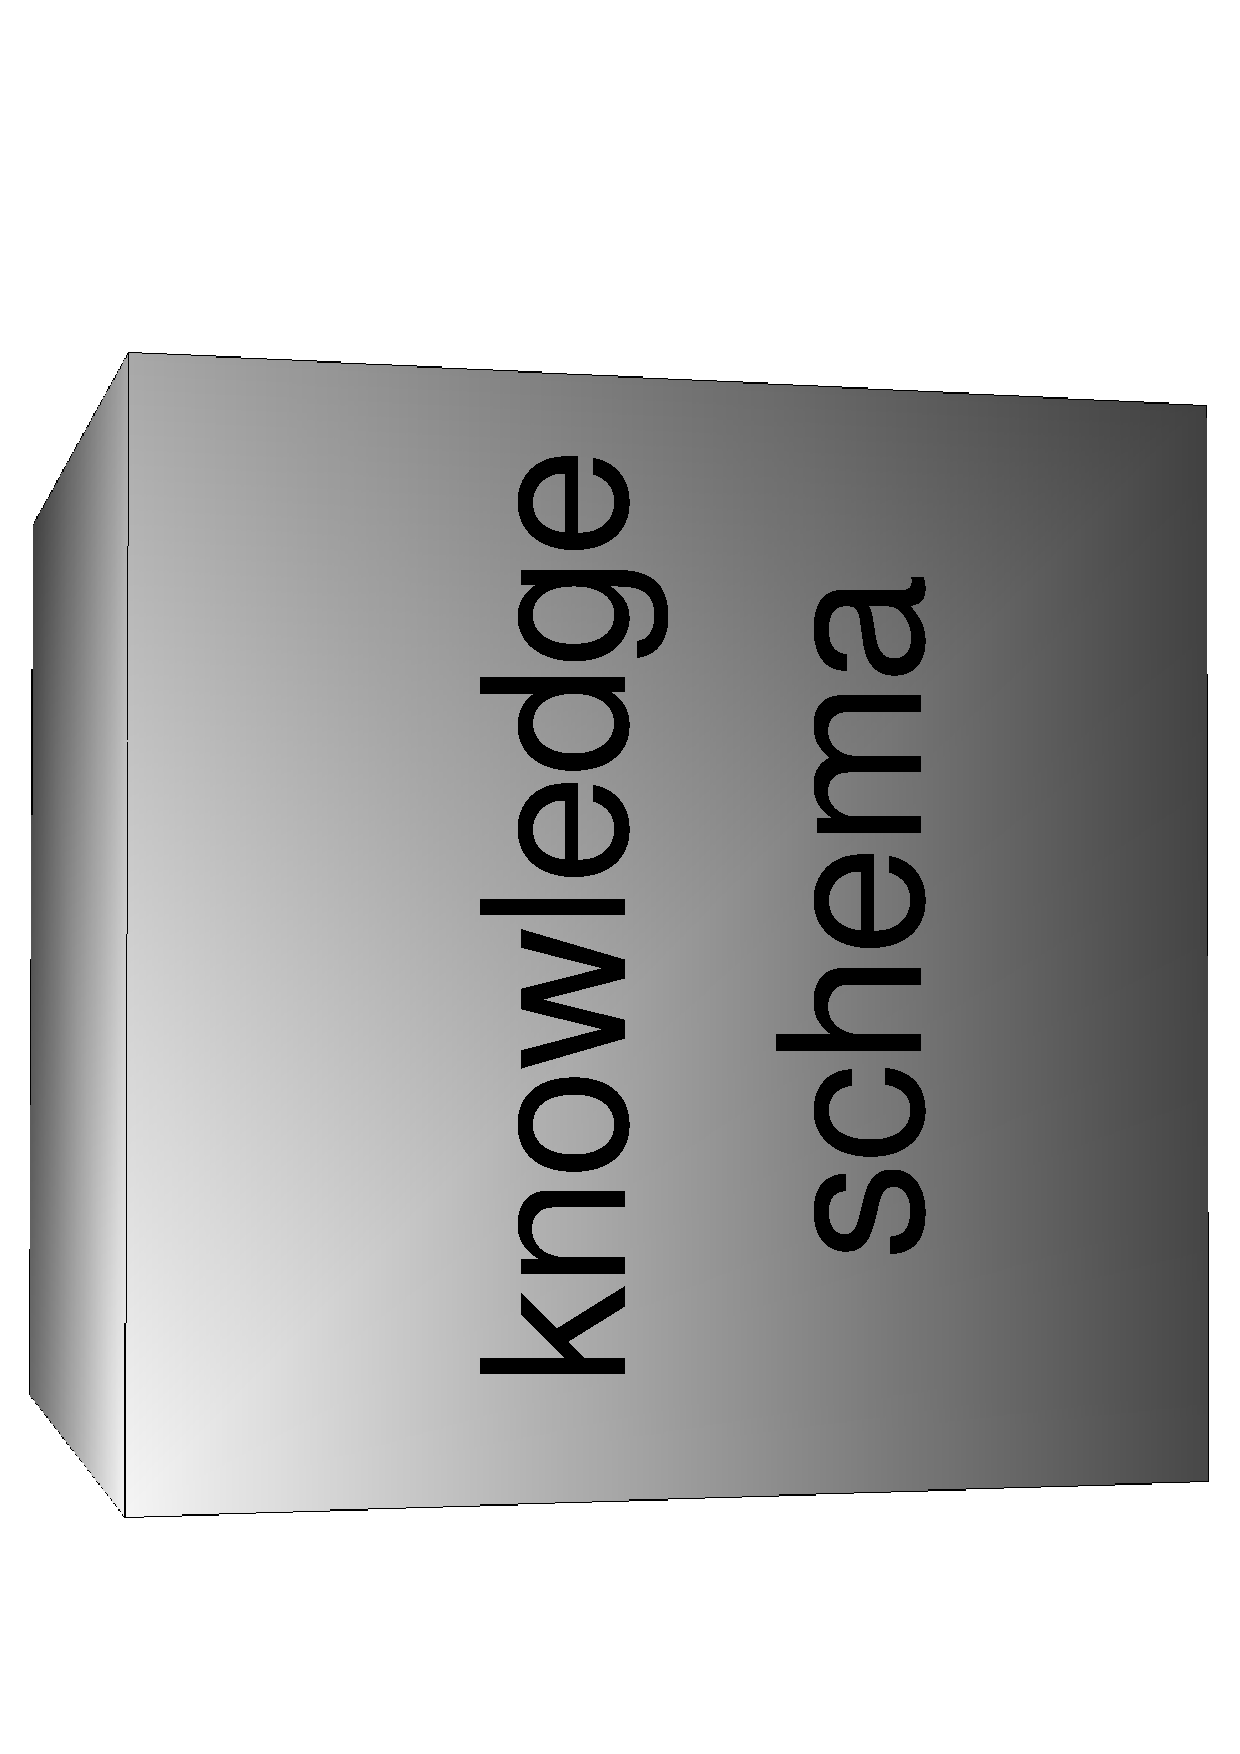
\includegraphics[scale=0.15,angle=-90]{graphic/contribution2.pdf}
\end{wrapfigure}

As first of the three main topics of part \ref{contribution_heading} of this
work, chapter \ref{statics_and_dynamics_heading} investigated why a separation
of static knowledge from its dynamic processing in a system is desirable. The
sections of this chapter deal with the \emph{Hierarchical Structuring} of
knowledge, in order to find a general schema for its modelling. After that,
chapter \ref{state_and_logic_heading} will elaborate on different kinds of
knowledge.
\vspace{1cm}

%
% $RCSfile: human_thinking.tex,v $
%
% Copyright (c) 2004. Christian Heller. All rights reserved.
%
% No copying, altering, distribution or any other actions concerning this
% document, except after explicit permission by the author!
% At some later point in time, this document is planned to be put under
% the GNU FDL license. For now, _everything_ is _restricted_ by the author.
%
% http://www.cybop.net
% - Cybernetics Oriented Programming -
%
% http://www.resmedicinae.org
% - Information in Medicine -
%
% @author Christian Heller <christian.heller@tuxtax.de>
%

\subsection{Human Thinking}
\label{human_thinking_heading}

The new classification is based on the idea of categorizing software patterns
after the principles of \emph{Human Thinking}, that is concepts of the logical
\emph{Mind}, as opposed to \emph{Artificial Neural Networks} (ANN) that want to
imitate the functioning of the physical \emph{Brain}.

The corresponding concepts were first introduced in \cite{heller2004}. After an
investigation of the fundamentals of human thinking, that is how human beings
understand their surrounding real world by abstracting it in \emph{Models}, that
paper concludes that there were three basic activities of abstraction:

\begin{enumerate}
    \item Discrimination
    \item Categorization
    \item Composition
\end{enumerate}

By discriminating their environment, humans are able to share it into discrete
\emph{Items}. Items with similar properties can be classified into a common super
\emph{Category}. Any abstract model of the universe is just an illusion, being
made up of yet smaller models, and nobody knows where this hierarchy really stops,
towards microcosm as well as towards macrocosm. Therefore, the third and last
kind of abstraction, namely composition, lets humans perceive the items in their
environment as \emph{Compound} of smaller items.

\begin{figure}[ht]
    \begin{center}
        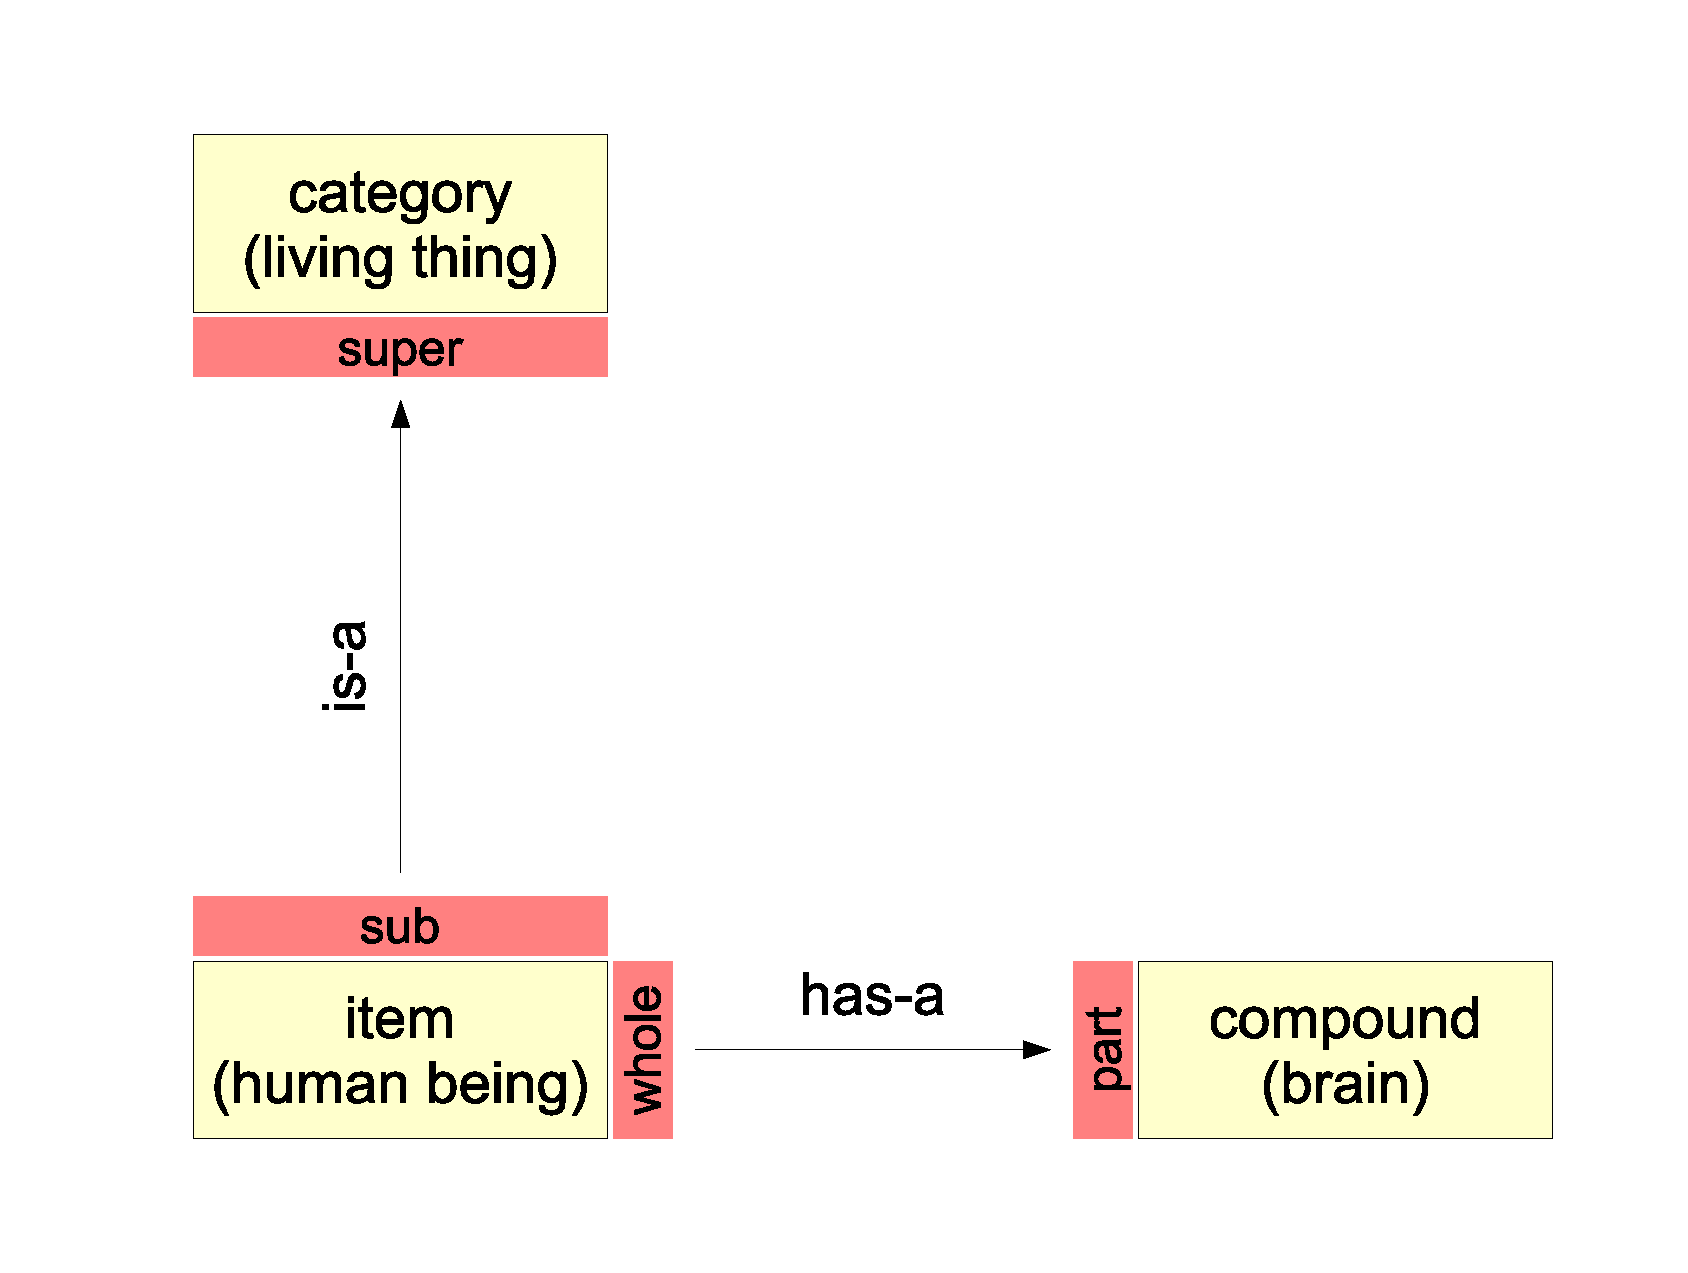
\includegraphics[scale=0.3]{vector/abstraction.eps}
        \caption{Abstractions of Human Thinking \cite{heller2004}}
        \label{abstraction_figure}
    \end{center}
\end{figure}

The latter two activities of abstraction -- categorization and composition --
are based on special \emph{Associations} (figure \ref{abstraction_figure}),
between a \emph{Super-} and a \emph{Sub} model and between a \emph{Whole-} and
a \emph{Part} model, respectively.

%
% $RCSfile: design_reflections.tex,v $
%
% Copyright (C) 2002-2008. Christian Heller.
%
% Permission is granted to copy, distribute and/or modify this document
% under the terms of the GNU Free Documentation License, Version 1.1 or
% any later version published by the Free Software Foundation; with no
% Invariant Sections, with no Front-Cover Texts and with no Back-Cover
% Texts. A copy of the license is included in the section entitled
% "GNU Free Documentation License".
%
% http://www.cybop.net
% - Cybernetics Oriented Programming -
%
% http://www.resmedicinae.org
% - Information in Medicine -
%
% Version: $Revision: 1.1 $ $Date: 2008-08-19 20:41:06 $ $Author: christian $
% Authors: Christian Heller <christian.heller@tuxtax.de>
%

\section{Design Reflections}
\label{design_reflections_heading}
\index{Design Reflections}

The previous sections investigated principles of human thinking, that is the
structures and relations used by the human mind to build abstract models of its
real world environment. The following sections focus on the impact of just
these principles on software design and suggest a number of changes while
rethinking state-of-the-art concepts.

%
% $RCSfile: pattern_systematics.tex,v $
%
% Copyright (C) 2002-2008. Christian Heller.
%
% Permission is granted to copy, distribute and/or modify this document
% under the terms of the GNU Free Documentation License, Version 1.1 or
% any later version published by the Free Software Foundation; with no
% Invariant Sections, with no Front-Cover Texts and with no Back-Cover
% Texts. A copy of the license is included in the section entitled
% "GNU Free Documentation License".
%
% http://www.cybop.net
% - Cybernetics Oriented Programming -
%
% http://www.resmedicinae.org
% - Information in Medicine -
%
% Version: $Revision: 1.1 $ $Date: 2008-08-19 20:41:08 $ $Author: christian $
% Authors: Christian Heller <christian.heller@tuxtax.de>
%

\subsection{Pattern Systematics}
\label{pattern_systematics_heading}
\index{Pattern Systematics}
\index{Software Pattern}
\index{Object Oriented Programming}
\index{OOP}
\index{Architectural Pattern}
\index{Design Pattern}
\index{Idiomatic Pattern}
\index{Human Thinking}
\index{Discrimination}
\index{Categorisation}
\index{Composition}
\index{Associations within Patterns}
\index{Itemisation Patterns}
\index{1:1 Association Patterns}
\index{1:n Association Patterns}
\index{Recursion Patterns}
\index{Bidirectionalism Patterns}
\index{Polymorphism Patterns}
\index{Grouping Patterns}
\index{Global Access Patterns}

\emph{Software Patterns} (section \ref{pattern_heading}) are a popular
architecture instrument of current systems and languages -- in the first line,
however, of \emph{Object Oriented Programming} (OOP) (section
\ref{object_oriented_programming_heading}). They describe design solutions that
belong to a higher conceptual level, as opposed to the programming paradigms
which are inherent to languages. A common criticism on the existence of
patterns is put into words by the free \emph{Wikipedia} encyclopedia
\cite{wikipedia} which writes:

\begin{quote}
    Some feel that the need for patterns results from using computer languages
    or techniques with insufficient abstraction ability. Under ideal factoring,
    a concept should \emph{not} be \emph{copied}, but merely \emph{referenced}.
    But if something is referenced instead of copied, then there is no pattern
    to label and catalog.
\end{quote}

In other words, patterns would become superfluous, if they could be applied
just \emph{once} to a system, in a manner that allowed any other parts of that
system to reference and reuse-, instead of copy them.

\emph{Cybernetics Oriented Programming} (CYBOP) wants to eliminate the need for
repeated pattern usage, and such enable application programmers, and possibly
even domain experts, to faster create better application systems. On the way to
reaching such sublime aims, a first step is to look at current pattern solutions
and try to identify what their common characteristics are. This was already
done in section \ref{pattern_heading}, which used traditional proposals
\cite{buschmann, gamma1995} to systematise patterns and divided them according
to the first categorisation level shown in figure \ref{pattern_figure}, into
\emph{Architectural-}, \emph{Design-} and \emph{Idiomatic} patterns.

This section proposes a \emph{new} systematics to classify software patterns.
It is based on the idea of classifying them after the principles of
\emph{Human Thinking}, as described in section \ref{human_thinking_heading}
before. These fundamental principles are: \emph{Discrimination},
\emph{Categorisation} and \emph{Composition}. Applied together, they may form
an abstract \emph{Schema} (introduced later, in section \ref{schema_heading}).

The latter two activities of abstraction -- categorisation and composition --
are based on special \emph{Associations} (figure \ref{abstraction_figure}),
between a \emph{Super-} and a \emph{Sub} model and between a \emph{Whole-} and
a \emph{Part} model, respectively. Most patterns heavily rely on associations,
too. This work therefore suggests to \cite{heller2005}: \textit{Take the kind
of association as criterion to sort patterns in a completely new way.}

\begin{table}[ht]
    \begin{center}
        \begin{footnotesize}
        \begin{tabular}{| p{20mm} | p{20mm} | p{50mm} | p{10mm} |}
            \hline
            \textbf{Category} & \textbf{Equivalent} & \textbf{Representative} & \textbf{Advice}\\
            \hline
            Itemisation & Discrimination & Command, Data Transfer Object, State, Memento, Envelope-Letter, Prototype & \vfill 
\includegraphics[scale=0.025,angle=-90]{graphic/happysmiley.pdf}\\
            \hline
            1:1 Association & Composition & Delegator, Object Adapter, Proxy (Surrogat, Client-/ Server Stub), Wrapper, Handle-Body, Bridge & \vfill 
\includegraphics[scale=0.025,angle=-90]{graphic/happysmiley.pdf}\\
            \hline
            1:n Association & Composition & Whole-Part, View Handler, Broker (Mediator), Master-Slave, Command Processor, Counted Pointer, Chain of Responsibility & \vfill 
\includegraphics[scale=0.025,angle=-90]{graphic/happysmiley.pdf}\\
            \hline
            Recursion & Composition & Composite, Interpreter, Decorator, Linked Wrapper & \vfill 
\includegraphics[scale=0.025,angle=-90]{graphic/happysmiley.pdf}\\
            \hline
            Bidirectionalism & -- & Observer (Callback, Publisher-Subscriber), Forwarder-Receiver, Chain of Responsibility, Visitor, Reflection & \vfill 
\includegraphics[scale=0.025,angle=-90]{graphic/sadsmiley.pdf}\\
            \hline
            Polymorphism & Categorisation & Template Method, Builder, Factory Method, Class Adapter, Abstract Factory (Kit), Strategy (Validator, Policy), Iterator (Cursor) & \vfill 
\includegraphics[scale=0.025,angle=-90]{graphic/serioussmiley.pdf}\\
            \hline
            Grouping & Categorisation & Layers, Domain Model, MVC & \vfill 
\includegraphics[scale=0.025,angle=-90]{graphic/happysmiley.pdf}\\
            \hline
            Global Access & -- & Singleton, Flyweight, Registry, Manager & \vfill 
\includegraphics[scale=0.025,angle=-90]{graphic/sadsmiley.pdf}\\
            \hline
        \end{tabular}
        \end{footnotesize}
        \caption{Pattern Systematics}
        \label{pattern_systematics_table}
    \end{center}
\end{table}

Table \ref{pattern_systematics_table} shows a systematics of the new pattern
categories with their equivalents in human thinking, some representative
example patterns and a recommendation for their usage in software engineering.
Patterns matching into more than one category are placed after the priority:
\emph{Recursion} over \emph{Polymorphism}.

%
% $RCSfile: recommendation.tex,v $
%
% Copyright (c) 2004. Christian Heller. All rights reserved.
%
% No copying, altering, distribution or any other actions concerning this
% document, except after explicit permission by the author!
% At some later point in time, this document is planned to be put under
% the GNU FDL license. For now, _everything_ is _restricted_ by the author.
%
% http://www.cybop.net
% - Cybernetics Oriented Programming -
%
% http://www.resmedicinae.org
% - Information in Medicine -
%
% @author Christian Heller <christian.heller@tuxtax.de>
%

\subsection{Recommendation}
\label{recommendation_heading}

The first category \emph{Itemization} (objectification) is the base of any
modelling activity and clearly necessary.

The next three categories \emph{1:1 Association}, \emph{1:n Association} and
\emph{Recursion} are special kinds of associations that rely exclusively on
\emph{unidirectional} relations and result in a clean architecture which is why
their usage is strongly recommended.

\emph{Bidirectionalism}, on the other hand, is an \emph{ill} variant of the three
aforementioned categories and should be avoided wherever possible. Patterns in
this category are one reason for endless loops and unpredictable behaviour since
it becomes very difficult to trace the effects that changes in one place of a
system have on others (section \ref{bidirectional_dependency_heading}).

\emph{Polymorphism} is a good thing. It relies on categorization and due to
inheritance can avoid a tremendous amount of otherwise redundant source code.
However, it also makes understanding a system more difficult, since the whole
architecture must be understood before being able to manipulate code correctly.
Unwanted source code changes caused by inheritance dependencies are often
described with the term \emph{Fragile Base Class Problem}
\cite[section \emph{Layers}]{buschmann}. They are just the opposite of what
inheritance was actually intended to be for: \emph{Reusability}
\cite[Vorwort]{gruhn}.

\emph{Grouping} models is essential to keep overview in a complex software
system. A very promising technology to support this are \emph{Ontologies}
\cite{hellerkunze}. A lot of thought-work has to go into them but if they are
well thought-out, they are clearly recommended.

The habit of globally accessing models is banned since OOP became popular.
However, it is not banned completely. Patterns like \emph{Singleton}
encapsulate and bundle global access but they still permit it. They disregard
any dependencies and relations in a system, such are a security risk and reason
for untraceable data changes. This paper sees the whole category of
\emph{Global Access} as potentially dangerous and can \emph{not} recommend its
patterns.

%
% $RCSfile: model_metamorphosis.tex,v $
%
% Copyright (C) 2002-2008. Christian Heller.
%
% Permission is granted to copy, distribute and/or modify this document
% under the terms of the GNU Free Documentation License, Version 1.1 or
% any later version published by the Free Software Foundation; with no
% Invariant Sections, with no Front-Cover Texts and with no Back-Cover
% Texts. A copy of the license is included in the section entitled
% "GNU Free Documentation License".
%
% http://www.cybop.net
% - Cybernetics Oriented Programming -
%
% http://www.resmedicinae.org
% - Information in Medicine -
%
% Version: $Revision: 1.1 $ $Date: 2008-08-19 20:41:07 $ $Author: christian $
% Authors: Christian Heller <christian.heller@tuxtax.de>
%

\subsection{Model Metamorphosis}
\label{model_metamorphosis_heading}
\index{Model Metamorphosis}
\index{Metamorphosis of Models}

One way to recognise the importance of \emph{Composition}, that is of models
with hierarchical character, is to compare several traditional modelling
approaches, as first suggested by Thomas Beale in \cite[p. 11-18]{archetypes}.
This \emph{Metamorphosis of Models} is empathised in the following paragraphs.

%
% $RCSfile: single_model.tex,v $
%
% Copyright (C) 2002-2008. Christian Heller.
%
% Permission is granted to copy, distribute and/or modify this document
% under the terms of the GNU Free Documentation License, Version 1.1 or
% any later version published by the Free Software Foundation; with no
% Invariant Sections, with no Front-Cover Texts and with no Back-Cover
% Texts. A copy of the license is included in the section entitled
% "GNU Free Documentation License".
%
% http://www.cybop.net
% - Cybernetics Oriented Programming -
%
% http://www.resmedicinae.org
% - Information in Medicine -
%
% Version: $Revision: 1.1 $ $Date: 2008-08-19 20:41:08 $ $Author: christian $
% Authors: Christian Heller <christian.heller@tuxtax.de>
%

\subsubsection{Single Model}
\label{single_model_heading}
\index{Single Model Approach}
\index{Entity Relationship Model}
\index{ERM}
\index{Object Oriented Model}
\index{OOM}
\index{Unified Modelling Language}
\index{UML}

Today, the most common design approach for standard application software is to
create a \emph{Single Model} of types whose semantics is often described in
form of an \emph{Entity Relationship-} (ER) or \emph{Object Oriented} (OO)
model,
%(section \ref{data_model_heading}),
the latter sometimes illustrated
using diagrams of the \emph{Unified Modeling Language} (UML).

\begin{figure}[ht]
    \begin{center}
        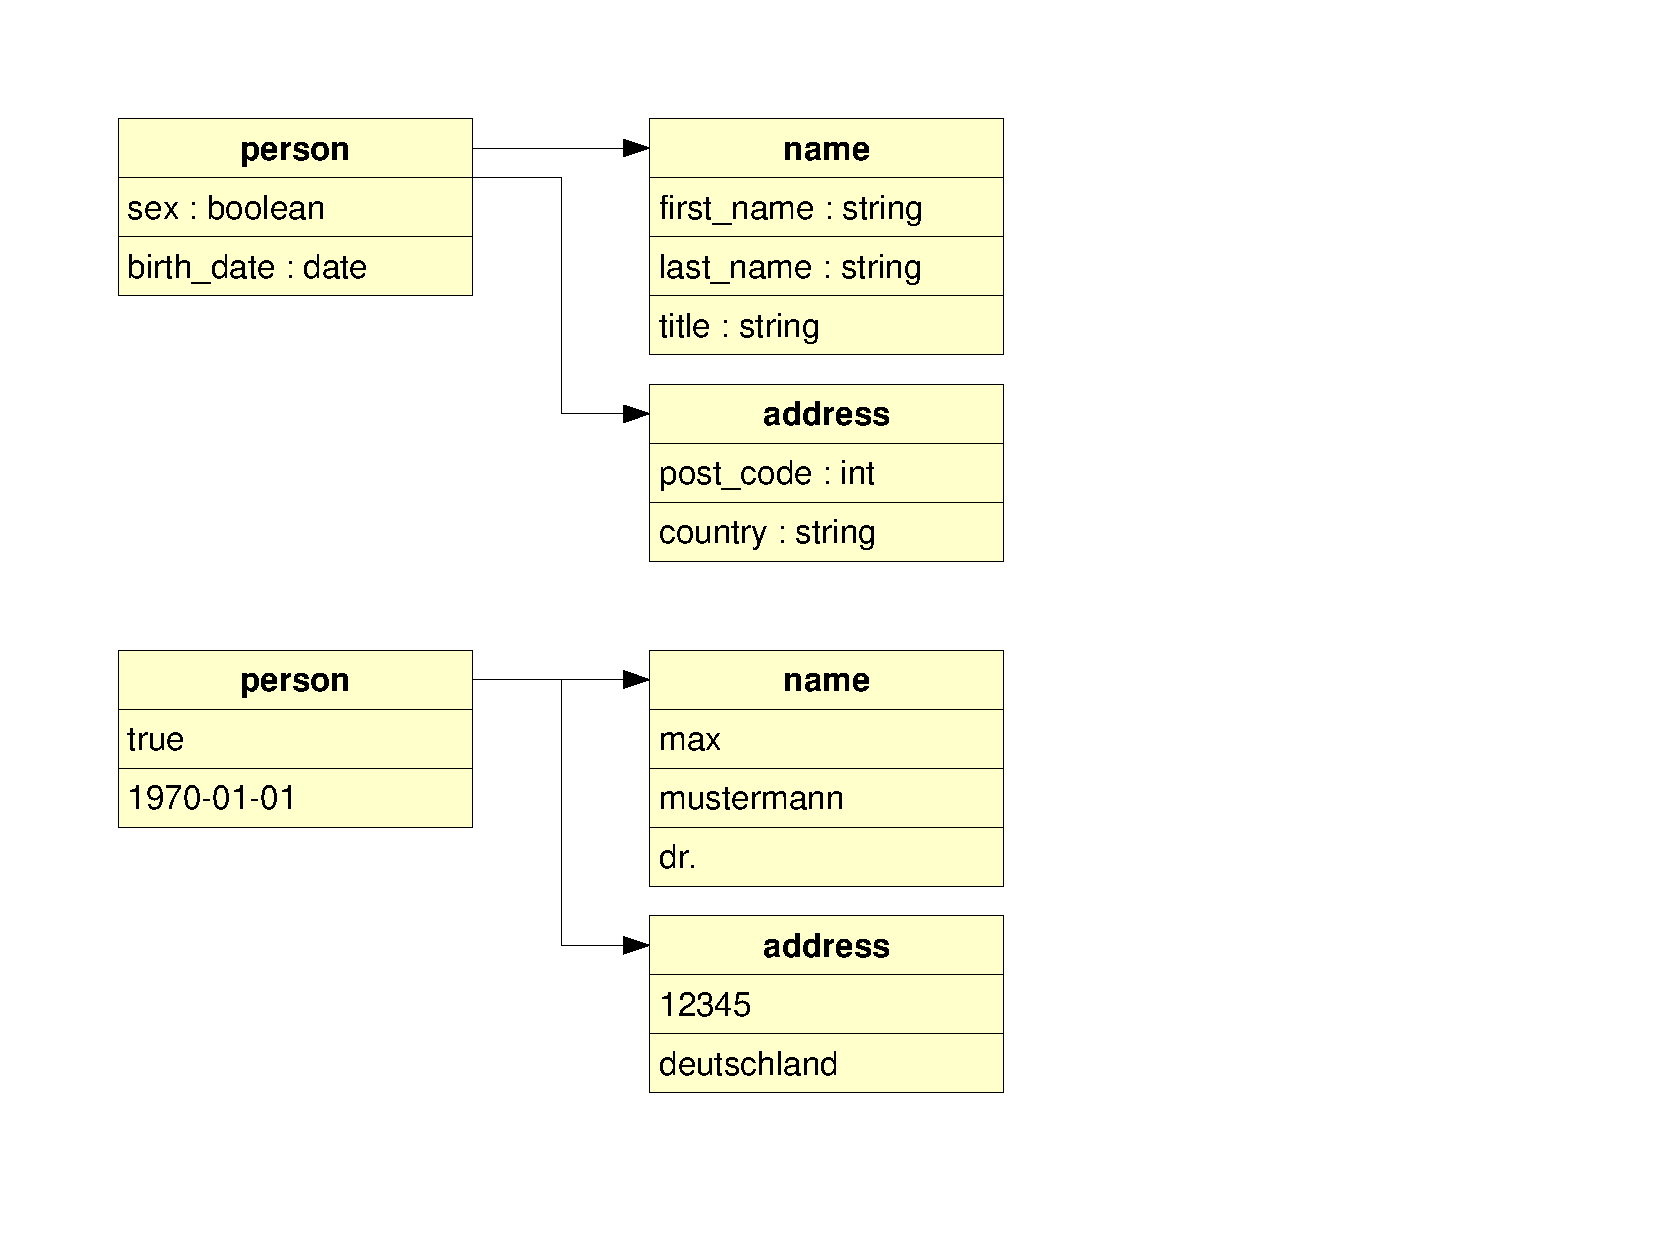
\includegraphics[scale=0.3,angle=-90]{graphic/single.pdf}
        \caption{Single Model Approach (adapted from \cite{archetypes})}
        \label{single_figure}
    \end{center}
\end{figure}

As example, figure \ref{single_figure} shows a UML \emph{Class Diagram} (CsD).
In its upper half, one can see a class \emph{Person} associated with the
classes \emph{Name} and \emph{Address}, as modelled at design time. They may be
part of a much larger model. The lower half of the figure shows the objects
(instances) at runtime, filled with concrete values. There are a number of
problems with this approach:

\input{inflexible_architecture}
\input{concept_mix}
\input{synchronisation_problems}
\input{complicated_processing}
\input{steady_upgrading}
\input{no_standardisation}

%
% $RCSfile: semi_structured_model.tex,v $
%
% Copyright (C) 2002-2008. Christian Heller.
%
% Permission is granted to copy, distribute and/or modify this document
% under the terms of the GNU Free Documentation License, Version 1.1 or
% any later version published by the Free Software Foundation; with no
% Invariant Sections, with no Front-Cover Texts and with no Back-Cover
% Texts. A copy of the license is included in the section entitled
% "GNU Free Documentation License".
%
% http://www.cybop.net
% - Cybernetics Oriented Programming -
%
% http://www.resmedicinae.org
% - Information in Medicine -
%
% Version: $Revision: 1.1 $ $Date: 2008-08-19 20:41:08 $ $Author: christian $
% Authors: Christian Heller <christian.heller@tuxtax.de>
%

\subsubsection{Semi Structured Model}
\label{semi_structured_model_heading}
\index{Semi Structured Model Approach}
\index{Named Values}
\index{Tagged Values}

A slightly improved version is the \emph{Semi Structured Model}. It relies on
the usage of \emph{Named Values} (sometimes called \emph{Tagged Values}), which
are stored in a dynamically extensible structure such as a list. That way,
future attributes can be added smoothly, without having to change the overall
model.

\begin{figure}[ht]
    \begin{center}
        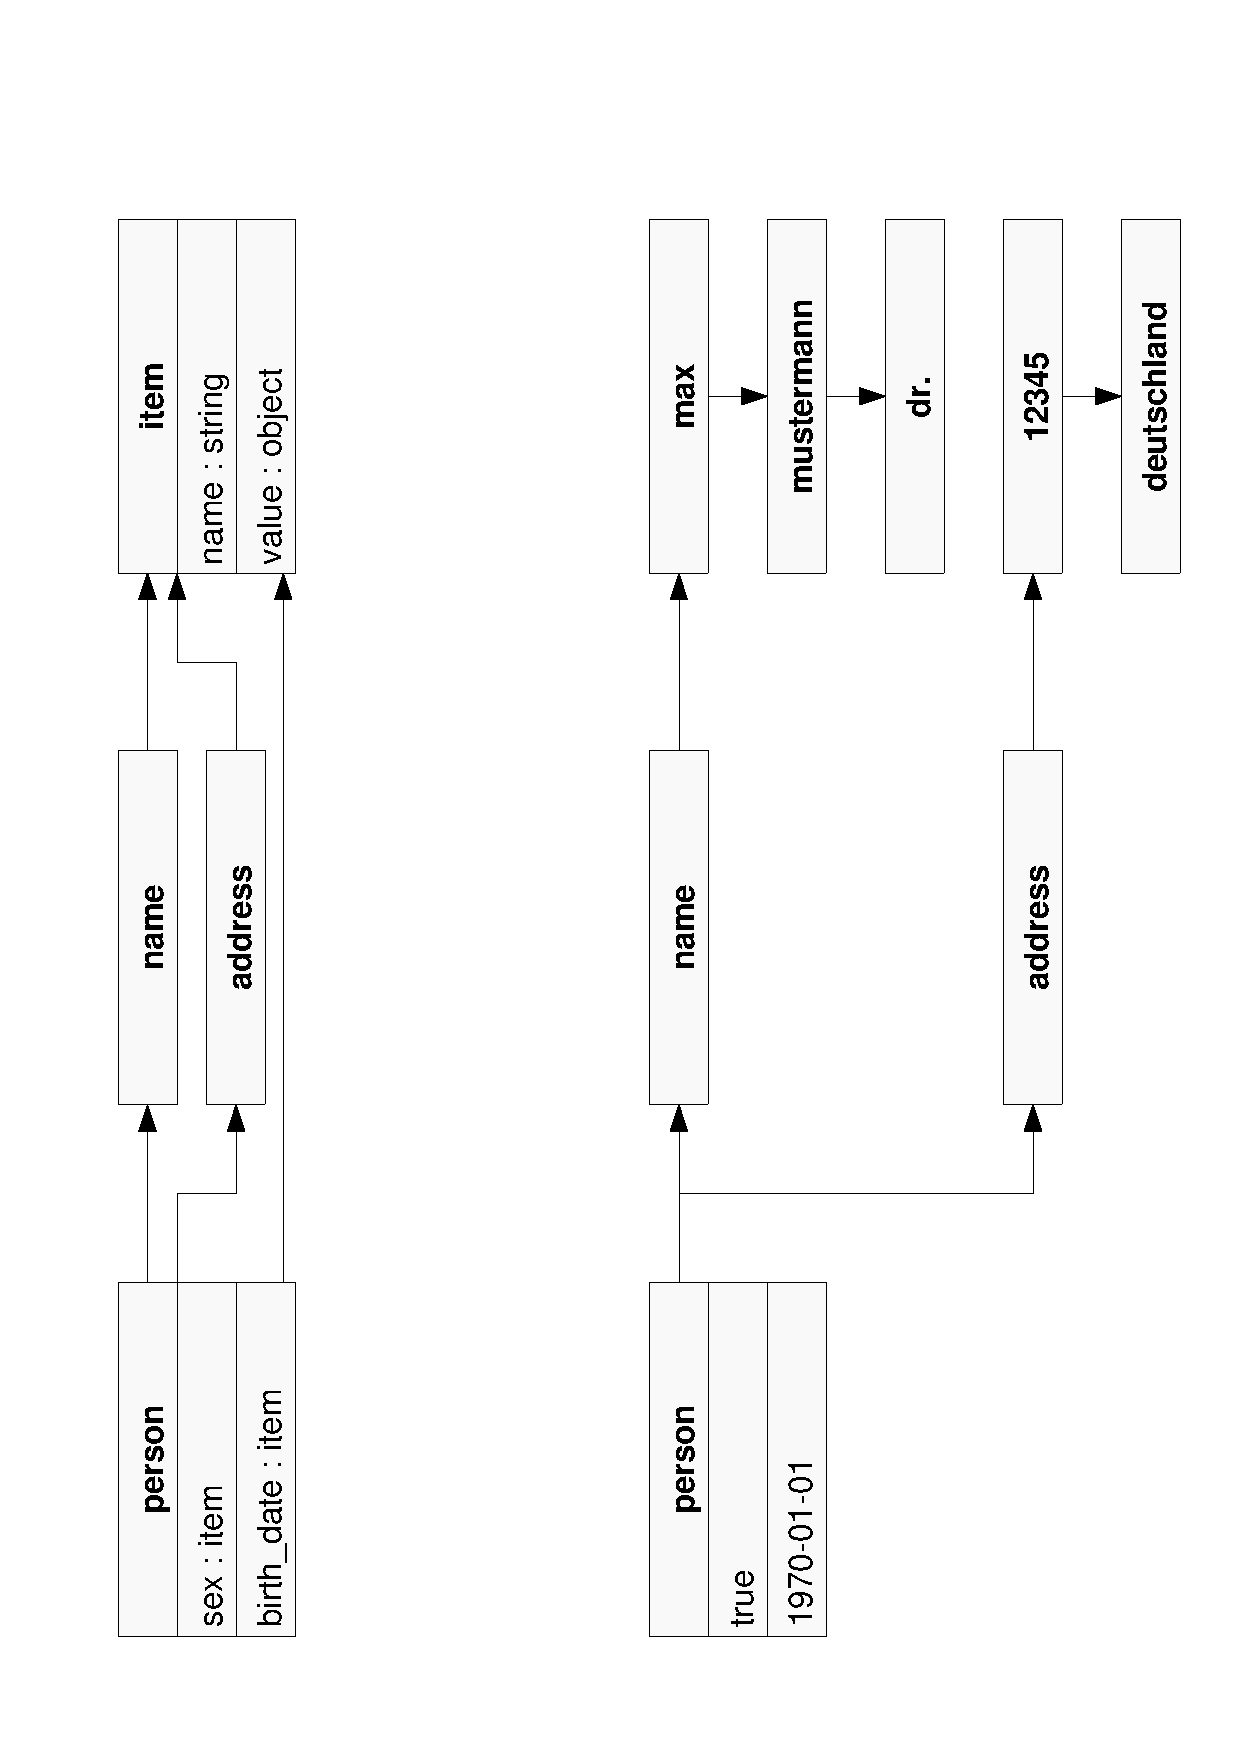
\includegraphics[scale=0.3,angle=-90]{graphic/semi.pdf}
        \caption{Semi Structured Model Approach (adapted from \cite{archetypes})}
        \label{semi_figure}
    \end{center}
\end{figure}

The example in figure \ref{semi_figure} shows a class \emph{Person} referencing
two linked lists, one called \emph{Name} and another called \emph{Address}. The
list elements are of type \emph{Item}. The dynamically extensible structure
becomes more obvious in the lower half of the figure, showing how the single
list elements reference each other. However, also here one can find
disadvantages \cite{archetypes}:

\begin{itemize}
    \item[-] Not all fields are dynamically changeable. Some are concrete
        attributes.
    \item[-] Only single lists of named values which do not allow for more
        complex internal structures are used.
    \item[-] Variability in structure is not generally dealt with.
    \item[-] Type information is lost for all list elements, since they are of
        one common type.
    \item[-] The system does not know anymore which elements are required.
\end{itemize}

%
% $RCSfile: hierarchical_model.tex,v $
%
% Copyright (C) 2002-2008. Christian Heller.
%
% Permission is granted to copy, distribute and/or modify this document
% under the terms of the GNU Free Documentation License, Version 1.1 or
% any later version published by the Free Software Foundation; with no
% Invariant Sections, with no Front-Cover Texts and with no Back-Cover
% Texts. A copy of the license is included in the section entitled
% "GNU Free Documentation License".
%
% http://www.cybop.net
% - Cybernetics Oriented Programming -
%
% http://www.resmedicinae.org
% - Information in Medicine -
%
% Version: $Revision: 1.1 $ $Date: 2008-08-19 20:41:07 $ $Author: christian $
% Authors: Christian Heller <christian.heller@tuxtax.de>
%

\subsubsection{Hierarchical Model}
\label{hierarchical_model_heading}
\index{Hierarchical Model Approach}
\index{Composition}
\index{Directed Acyclical Graph}
\index{DAG}
\index{Composite Pattern}

The \emph{Hierarchical Model} as yet more generalised form of data representation
is based on \emph{Composition} as one of the principles of human thinking
(section \ref{abstraction_heading}). Its tree structure -- ideally in form of a
\emph{Directed Acyclical Graph} (DAG) (section \ref{terminology_heading}) --
allows dynamic extensions of data types, by simply adding child nodes (parts)
to a parent node (whole), in the knowledge tree.

\begin{figure}[ht]
    \begin{center}
        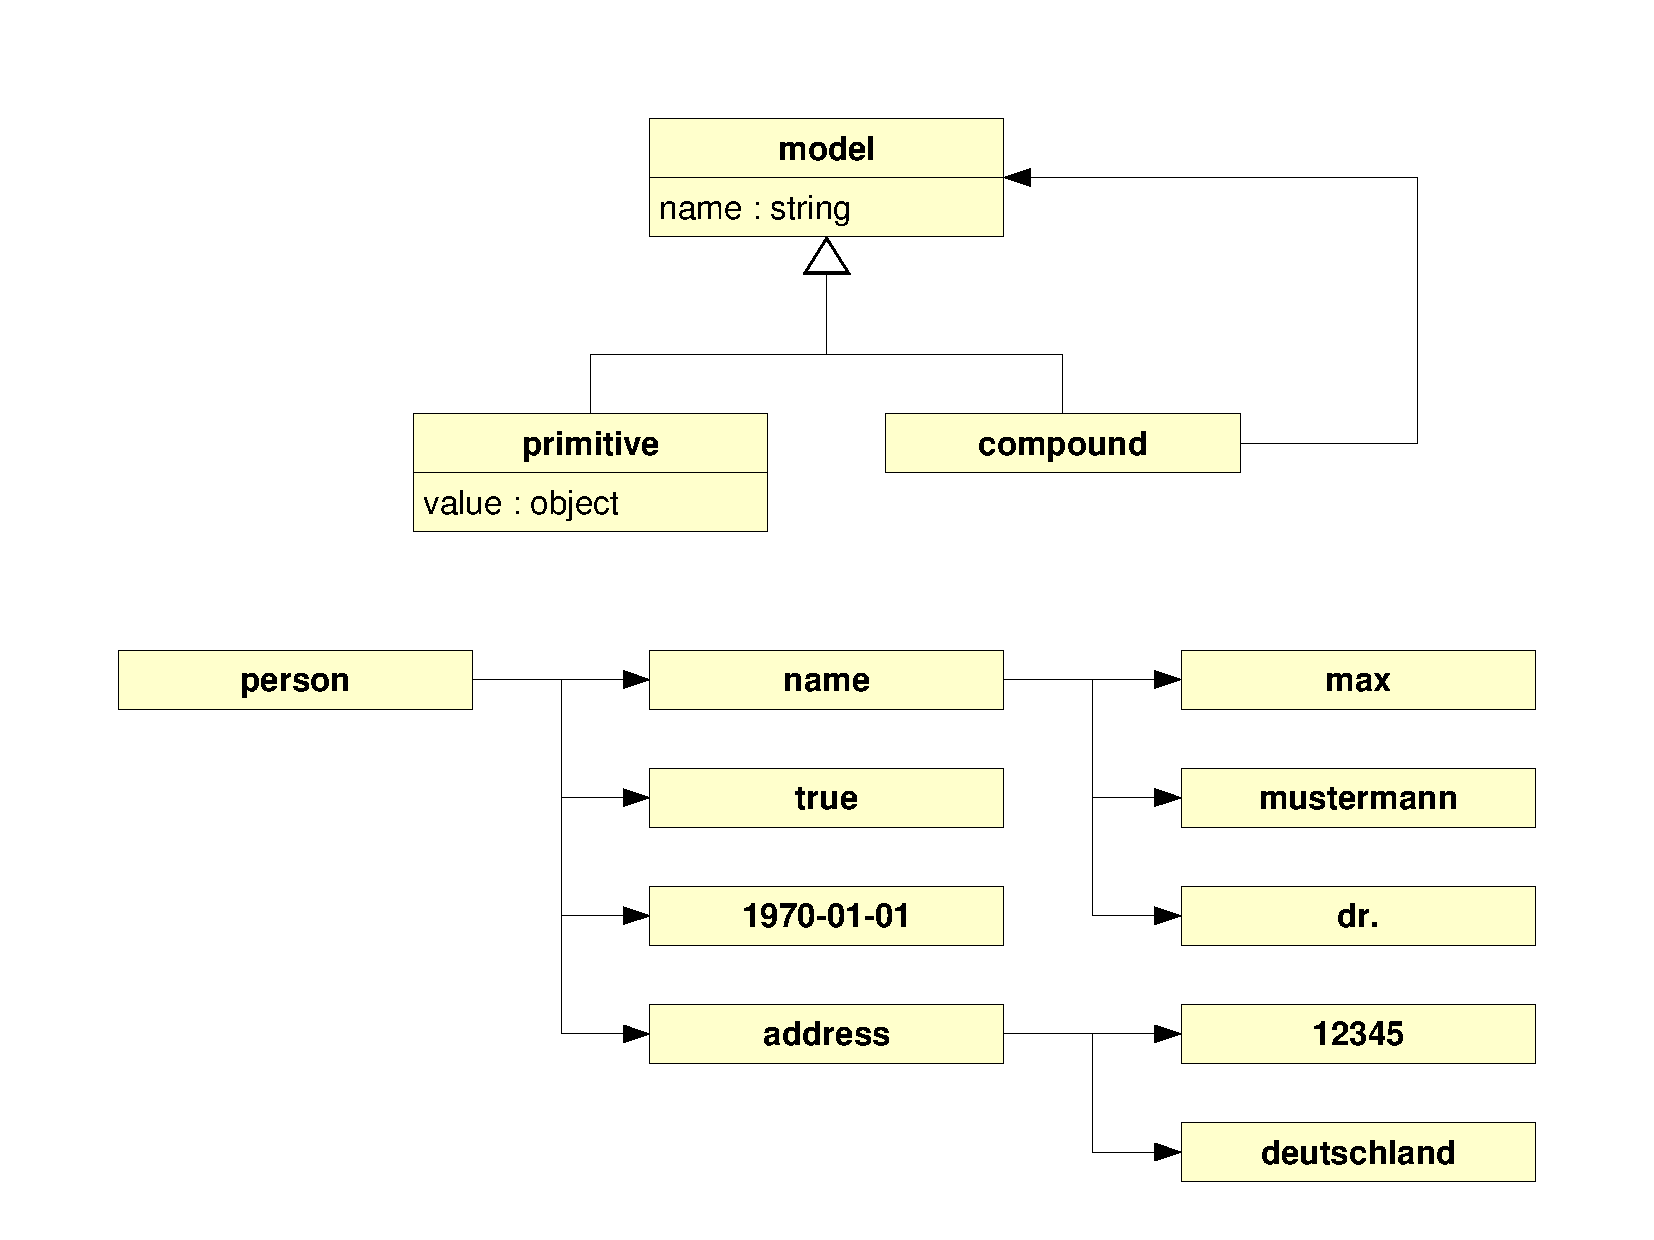
\includegraphics[scale=0.3,angle=-90]{graphic/hierarchical.pdf}
        \caption{Hierarchical Model Approach (adapted from \cite{archetypes})}
        \label{hierarchical_figure}
    \end{center}
\end{figure}

The upper half of figure \ref{hierarchical_figure} shows the \emph{Composite}
software pattern (section \ref{composite_heading}). Its classes do not contain
hard-coded attributes; two exceptions are the \emph{Primitive} class' attribute
\emph{value} and the \emph{Compound} class' dynamically extensible structure.
The structure may be a list, and it stores all of the compound's parts in it.
Parts may be primitiva or compounds themselves. As already proposed by the
\emph{Semi Structured Model} before, each part is identified by a name that is
unique within its compound. The diagram in the lower half of the figure clearly
shows the hierarchical tree structure of runtime instances.

The only open issue when using purely hierarchical models is that the semantics
-- the actual domain concepts -- is lost. Knowledge models, together with their
parts and meta information about these (position, size, colour, constraints --
as described in section \ref{human_thinking_heading}), thus need to be defined
somewhere else. The later section \ref{knowledge_representation_heading}
proposes a generic knowledge schema for doing this.


%
% $RCSfile: structure_by_hierarchy.tex,v $
%
% Copyright (C) 2002-2008. Christian Heller.
%
% Permission is granted to copy, distribute and/or modify this document
% under the terms of the GNU Free Documentation License, Version 1.1 or
% any later version published by the Free Software Foundation; with no
% Invariant Sections, with no Front-Cover Texts and with no Back-Cover
% Texts. A copy of the license is included in the section entitled
% "GNU Free Documentation License".
%
% http://www.cybop.net
% - Cybernetics Oriented Programming -
%
% http://www.resmedicinae.org
% - Information in Medicine -
%
% Version: $Revision: 1.1 $ $Date: 2008-08-19 20:41:09 $ $Author: christian $
% Authors: Christian Heller <christian.heller@tuxtax.de>
%

\subsection{Structure by Hierarchy}
\label{structure_by_hierarchy_heading}
\index{Structure by Hierarchy}
\index{Composition}
\index{Knowledge Model}
\index{Domain Model}
\index{Artificial Intelligence}
\index{AI}
\index{Knowledge Engineering}
\index{Omnipresence of Hierarchy}
\index{Model View Controller Pattern}
\index{MVC}
\index{Hierarchical Model View Controller Pattern}
\index{HMVC}
\index{Tree}

The principle of \emph{Composition} not only allows the creation of highly
flexible models, the \emph{Hierarchies} it makes up allow humans to combine
several concepts in a common, greater model. \emph{Structure by Hierarchy} as
idea has been applied to numerous \emph{Knowledge-} and \emph{Domain Models},
especially in the fields of \emph{Artificial Intelligence} (AI) and
\emph{Knowledge Engineering} (section \ref{knowledge_engineering_heading}). But
obviously, it has not been used for the design of \emph{complete} systems yet,
even though this seems quite logical.

To demonstrate the omnipresence of \emph{Hierarchies} in a system, the parts of
the \emph{Model View Controller} (MVC) software pattern described in section
\ref{model_view_controller_heading} shall be considered once again. The MVC is
a very representative example as it is used in one or another form by a
majority of systems, today.

\begin{figure}[ht]
    \begin{center}
        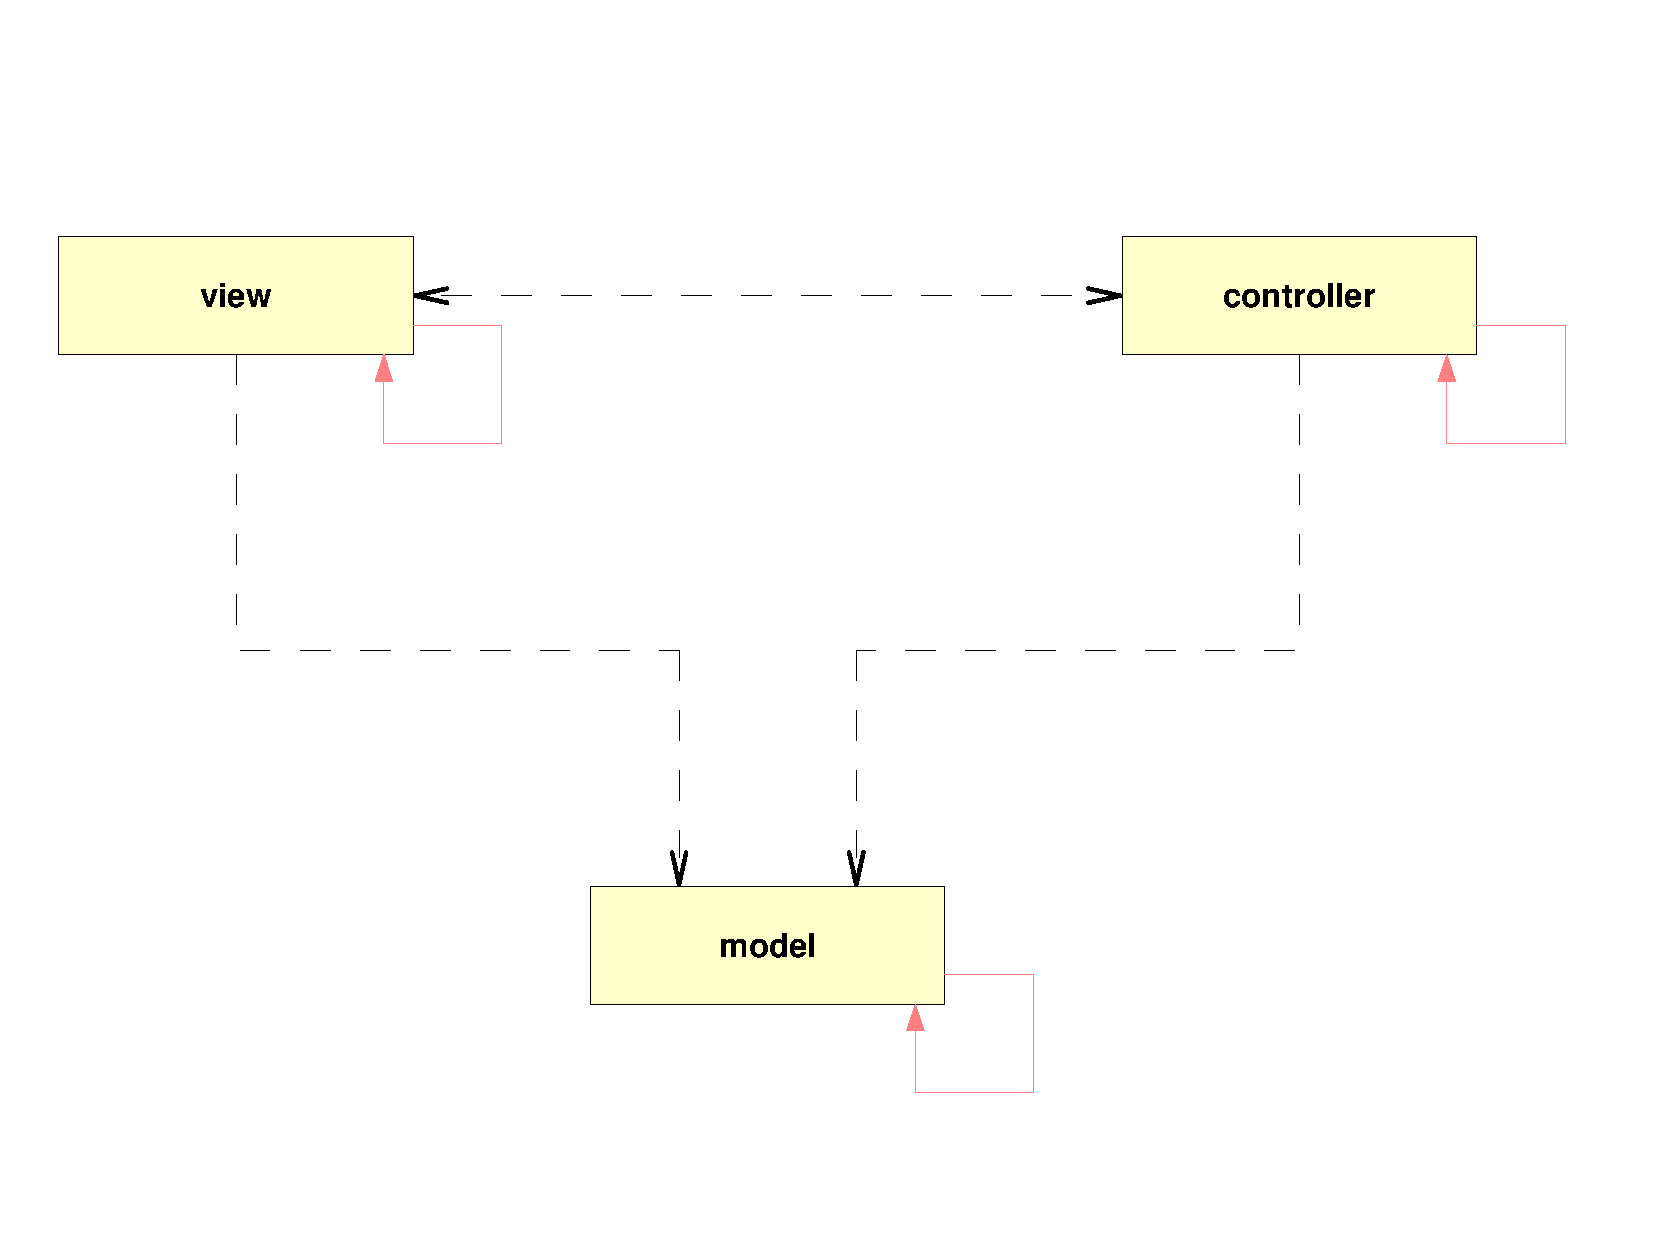
\includegraphics[scale=0.3,angle=-90]{graphic/adapted.pdf}
        \caption{Adapted (H)MVC Pattern with Hierarchical Elements}
        \label{adapted_figure}
    \end{center}
\end{figure}

The MVC pattern (figure \ref{adapted_figure}) consists of a \emph{View} that is
mostly implemented as \emph{Graphical User Interface} (GUI) frame with panel,
menubar, menu items and smaller components which, in this order, are all part
of the frame's hierarchy. Then, there is the \emph{Controller}. The
\emph{Hierarchical Model View Controller} (HMVC) pattern (section
\ref{hierarchical_model_view_controller_heading}) suggested to use a controller
hierarchy consisting of \emph{MVC Triads}. Finally, there is the \emph{Model}
of domain concepts which not only knowledge systems can structure
hierarchically. Reflecting these facts, one question is at hand:

\begin{quote}
    If View, Controller and Model ideally have a hierarchical structure,\\
    why not creating whole software systems after this paradigm?\\
    Isn't every system, in essence, just a \emph{Tree} of items?
\end{quote}

%
% $RCSfile: association_elimination.tex,v $
%
% Copyright (C) 2002-2008. Christian Heller.
%
% Permission is granted to copy, distribute and/or modify this document
% under the terms of the GNU Free Documentation License, Version 1.1 or
% any later version published by the Free Software Foundation; with no
% Invariant Sections, with no Front-Cover Texts and with no Back-Cover
% Texts. A copy of the license is included in the section entitled
% "GNU Free Documentation License".
%
% http://www.cybop.net
% - Cybernetics Oriented Programming -
%
% http://www.resmedicinae.org
% - Information in Medicine -
%
% Version: $Revision: 1.1 $ $Date: 2008-08-19 20:41:05 $ $Author: christian $
% Authors: Christian Heller <christian.heller@tuxtax.de>
%

\subsection{Association Elimination}
\label{association_elimination_heading}
\index{Association Elimination}
\index{Hierarchy as Principle}
\index{Ontology}
\index{Electronic Health Record}
\index{EHR}
\index{Episode Based EHR}
\index{Object Oriented Programming}
\index{OOP}
\index{Super Model}
\index{Sub Model}
\index{Granularity of Items}
\index{Unidirectional Dependency}
\index{Eliminated Sub Associations}
\index{Ontological Level}
\index{Layers of a System}
\index{Top-most Super Category}

To pursue the idea of a purely hierarchical software system, it seems useful to
investigate in which way domain data models can get simplified. This section
therefore demonstrates how the principle of \emph{Hierarchy} may be applied to
obtain an \emph{Ontology} \cite{hellerkunze}.

\begin{figure}[ht]
    \begin{center}
        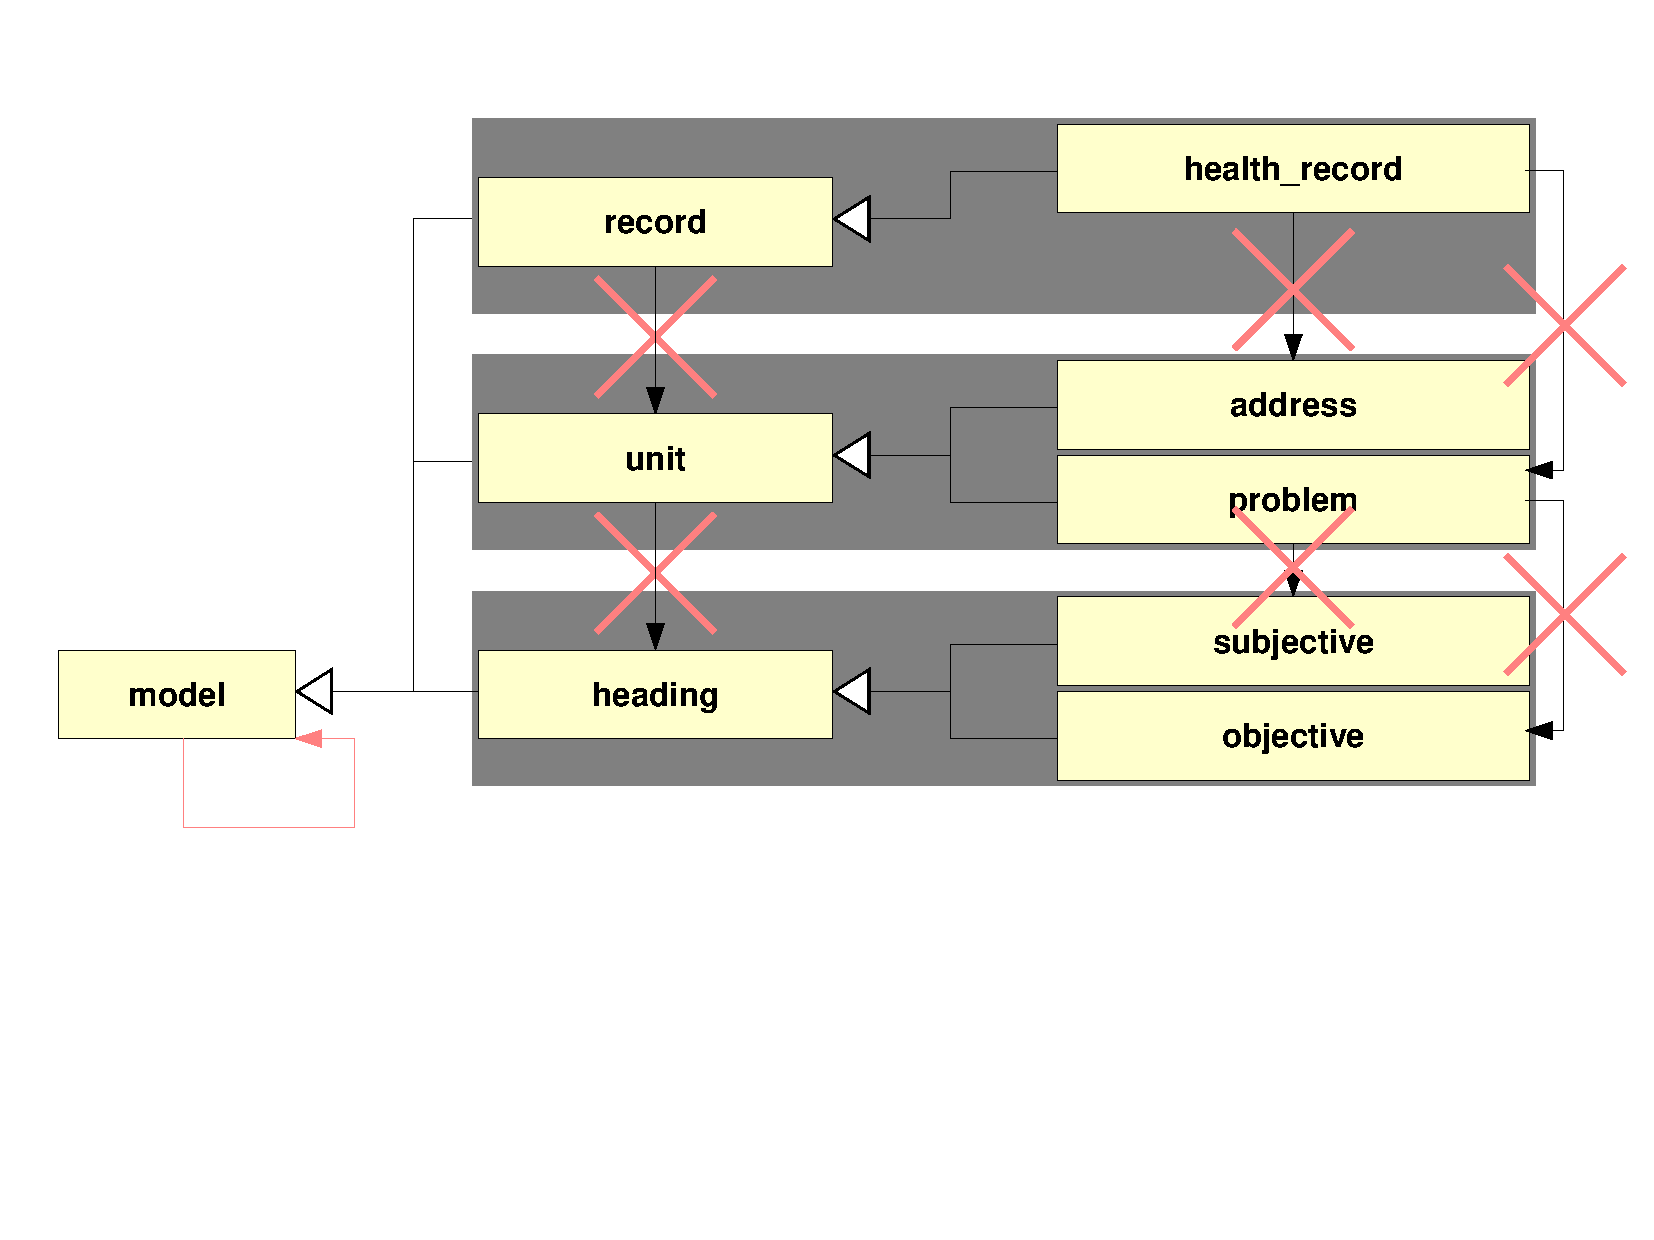
\includegraphics[scale=0.3,angle=-90]{graphic/elimination.pdf}
        \caption{Association Elimination in an EHR}
        \label{elimination_figure}
    \end{center}
\end{figure}

An \emph{Electronic Health Record} (EHR) will serve as example domain model,
whose simplified structure is shown in figure \ref{elimination_figure}. It
consists of numerous parts whereof two may be \emph{Address} and \emph{Problem}.
Following the \emph{Episode-based EHR} recommendation \cite{westerhof},
\emph{Problem} may, besides others, consist of parts of type \emph{Subjective}
and \emph{Objective}. All these associations between part models are needed to
navigate through the overall domain model.

A frequent design decision in classical \emph{Object Oriented Programming}
(OOP) is to sum up common properties of \emph{Sub} models by introducing a
\emph{Super} model (category). It should never be \emph{Properties}, but rather
the \emph{Granularity} of objects leading to the creation of a super category,
as the later section \ref{categorisation_versus_composition_heading} will
recommend. The \emph{OpenEHR} project \cite{openehr} suggests to let the
above-mentioned sub models inherit from the more coarse-grained super
categories \emph{Record}, \emph{Unit} and \emph{Heading}.

Whichever reason -- once the super categories are there, they should be
associated similarly to their sub categories, that is in the same direction,
using solely \emph{unidirectional} dependencies. (The problematic nature of
bidirectional dependencies was elaborated in section \ref{pattern_heading}.)
Afterwards, all associations between sub categories become superfluous as every
sub category can reach its sibling across the super categories' association
(figure \ref{elimination_figure}). In other words:
\emph{Super- eliminate Sub Associations}.

Here a short Java code example for how the \emph{HealthRecord} may retrieve a
reference to \emph{Address}:

\begin{scriptsize}
    \begin{verbatim}
    Address a = (Address) get_element("address");
    \end{verbatim}
\end{scriptsize}

\emph{HealthRecord} inherits the \emph{get\_element} method from its super
category \emph{Record}. \emph{Record} holds differing sub models of category
\emph{Unit} and other instances. The \emph{get\_element} method delivers back
a general \emph{Model} that still needs to be down-casted to the expected sub
category \emph{Address}.

\begin{figure}[ht]
    \begin{center}
        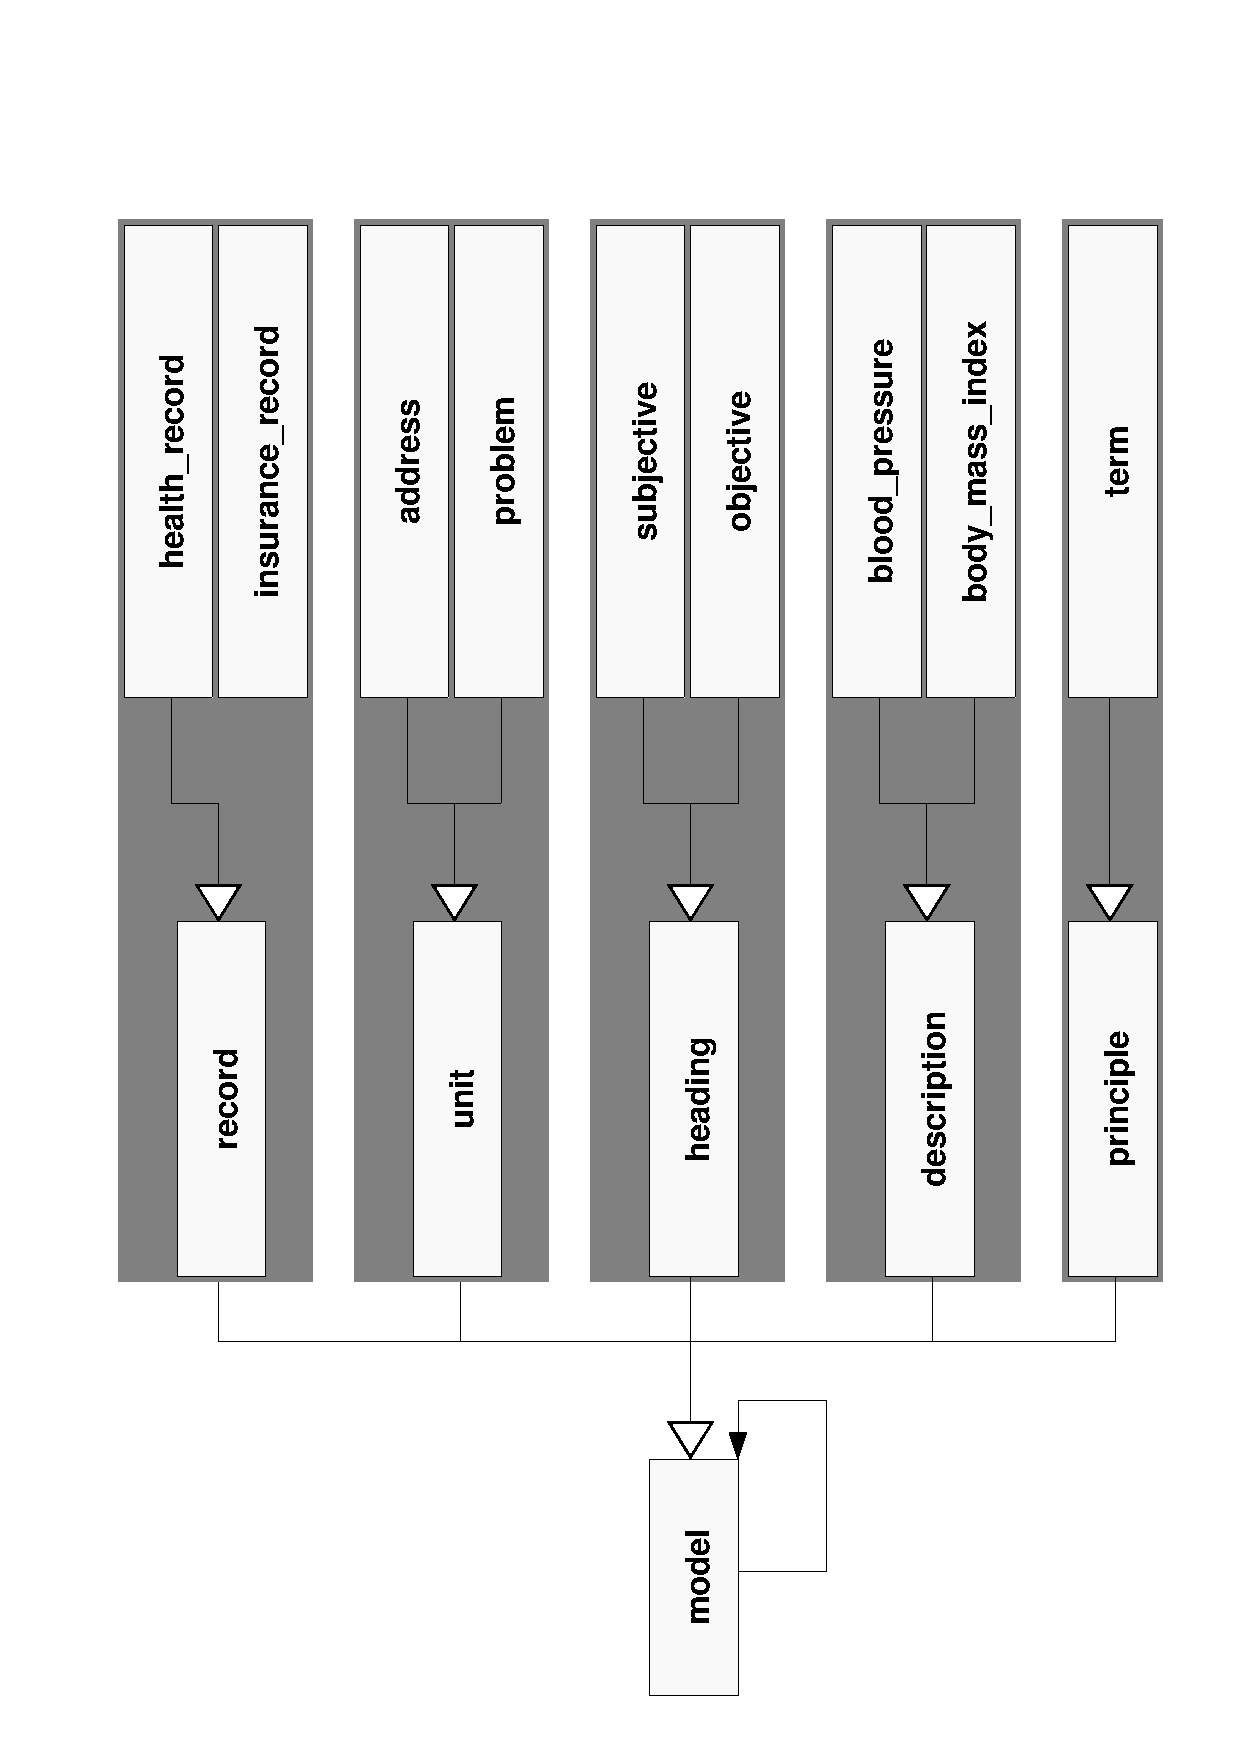
\includegraphics[scale=0.3,angle=-90]{graphic/levels.pdf}
        \caption{Model Container and Ontological Levels}
        \label{levels_figure}
    \end{center}
\end{figure}

The definition of models, their dependencies (defined by associations) and
granularities (defined by inheritance) in a software system results in several
\emph{Layers} of models of common granularity (figure \ref{levels_figure}).
These layers are often called \emph{Ontological Level} as they, together, form
an \emph{Ontology} (sections \ref{ontology_heading},
\ref{knowledge_ontology_heading}).

An ontology of that kind can, of course, be created for every knowledge model.
The financial sector -- like an insurance company, for example -- may use an
\emph{Insurance Record} with comparable structure.

The idea to structure software as a system of \emph{Layers} was also suggested
by the equally named pattern in section \ref{layers_heading}. The difference
between the two is that the \emph{Layers} pattern divides a system only by its
\emph{Functionality}, for example into \emph{User Interface}, \emph{Domain},
\emph{Data Mapper} and \emph{Data Source}. An \emph{Ontology} additionally
groups model items by their \emph{Granularity}. By inheriting from a common
superior category, sub categories indicate that they logically belong to the
same \emph{Layer}.

Continuing the structuring process of introducing more and more common super
categories, for all equally-granular items, the development culminates in one
top-most super category of all other categories in the system, which this paper
calls \emph{Model}. It is as general as the \emph{java.lang.Object} class for
the Java class library \cite{java}, only that it additionally represents a
\emph{Container} that can store models of any category, as explained in
\cite{hellerbohl}. In other words, \emph{Model} provides the meta functionality
of a container behaviour to \emph{all} other categories in a system.

%
% $RCSfile: hierarchical_algorithm.tex,v $
%
% Copyright (C) 2002-2008. Christian Heller.
%
% Permission is granted to copy, distribute and/or modify this document
% under the terms of the GNU Free Documentation License, Version 1.1 or
% any later version published by the Free Software Foundation; with no
% Invariant Sections, with no Front-Cover Texts and with no Back-Cover
% Texts. A copy of the license is included in the section entitled
% "GNU Free Documentation License".
%
% http://www.cybop.net
% - Cybernetics Oriented Programming -
%
% http://www.resmedicinae.org
% - Information in Medicine -
%
% Version: $Revision: 1.1 $ $Date: 2008-08-19 20:41:07 $ $Author: christian $
% Authors: Christian Heller <christian.heller@tuxtax.de>
%

\subsection{Hierarchical Algorithm}
\label{hierarchical_algorithm_heading}
\index{Hierarchical Algorithm}

Of course, algorithms, workflows and other activities over time can be
structured hierarchically as well.

\begin{figure}[ht]
    \begin{center}
        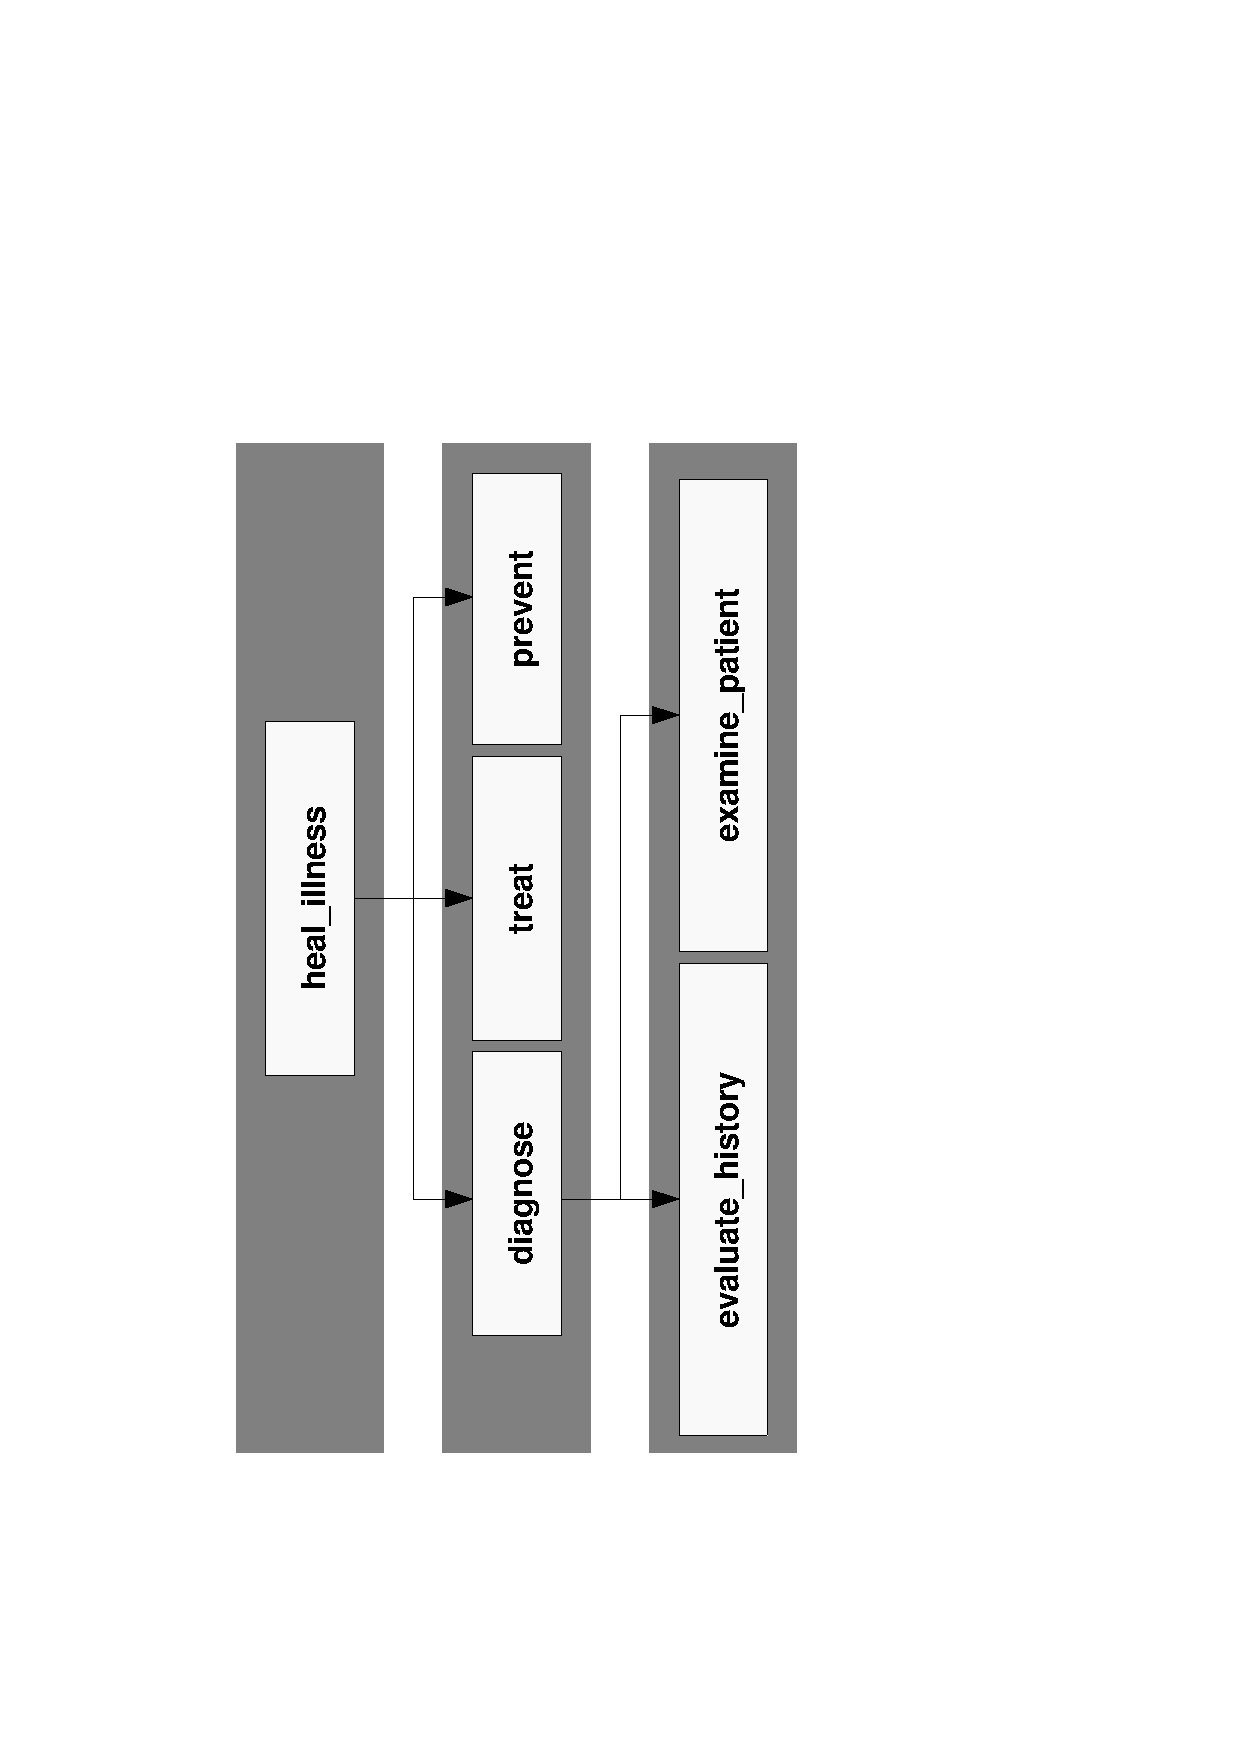
\includegraphics[scale=0.3,angle=-90]{graphic/algorithm.pdf}
        \caption{\emph{Heal Illness} as Hierarchical Algorithm, taken from Medicine}
        \label{algorithm_figure}
    \end{center}
\end{figure}

To stick with the domain of medicine: A \emph{Medical Doctor}'s (MD) activity
is to \emph{Heal an Illness}. Part processes the MD has to carry out commonly
are to \emph{Diagnose}, to \emph{Treat} and to \emph{Prevent} an illness
(figure \ref{algorithm_figure}). Further structurings are possible. To the
process of diagnostics belong activities like \emph{Evaluate History} or
\emph{Examine Patient}.

%
% $RCSfile: framework_example.tex,v $
%
% Copyright (C) 2002-2008. Christian Heller.
%
% Permission is granted to copy, distribute and/or modify this document
% under the terms of the GNU Free Documentation License, Version 1.1 or
% any later version published by the Free Software Foundation; with no
% Invariant Sections, with no Front-Cover Texts and with no Back-Cover
% Texts. A copy of the license is included in the section entitled
% "GNU Free Documentation License".
%
% http://www.cybop.net
% - Cybernetics Oriented Programming -
%
% http://www.resmedicinae.org
% - Information in Medicine -
%
% Version: $Revision: 1.1 $ $Date: 2008-08-19 20:41:06 $ $Author: christian $
% Authors: Christian Heller <christian.heller@tuxtax.de>
%

\subsection{Framework Example}
\label{framework_example_heading}
\index{Framework Example}
\index{Reference Information Model}
\index{RIM}
\index{Health Level Seven}
\index{HL7}
\index{Single Model Approach}
\index{Object Oriented Programming}
\index{OOP}
\index{Top Level Container}
\index{Access Method Elimination}
\index{Knowledge Specification}
\index{Encapsulation}

A much more complex example than the EHR structure demonstrated in section
\ref{association_elimination_heading} is the \emph{Reference Information Model}
(RIM) framework of the \emph{Health Level Seven} (HL7) standardisation
organisation (chapter \ref{res_medicinae_heading}). It is a quite typical
software model, developed in a \emph{Single Model Approach} (section
\ref{single_model_heading}), as it may similarly exist in other business areas.
The coloured legend in figure \ref{rim_figure} helps distinguish the various
parts of the RIM. The part to be picked out to have a closer look here is the
several kinds of RIM \emph{Entities} (figure \ref{entity_figure}).

Diving yet deeper into the framework, one will find the \emph{Person} class,
being a sub class of \emph{Living Subject} (figure \ref{person_figure}). Since
the RIM is an \emph{Object Oriented} (OO) framework, each class will probably
have access methods for all of its attributes. For the \emph{Person} class, the
access methods for \emph{birthdate} and \emph{address} are shown in the figure.
The right-hand side also shows the typical one-line contents of the \emph{set}/
\emph{get} methods, although more code may be put into them, for reasons of
notification, update or others more.

\begin{figure}[ht]
    \begin{center}
        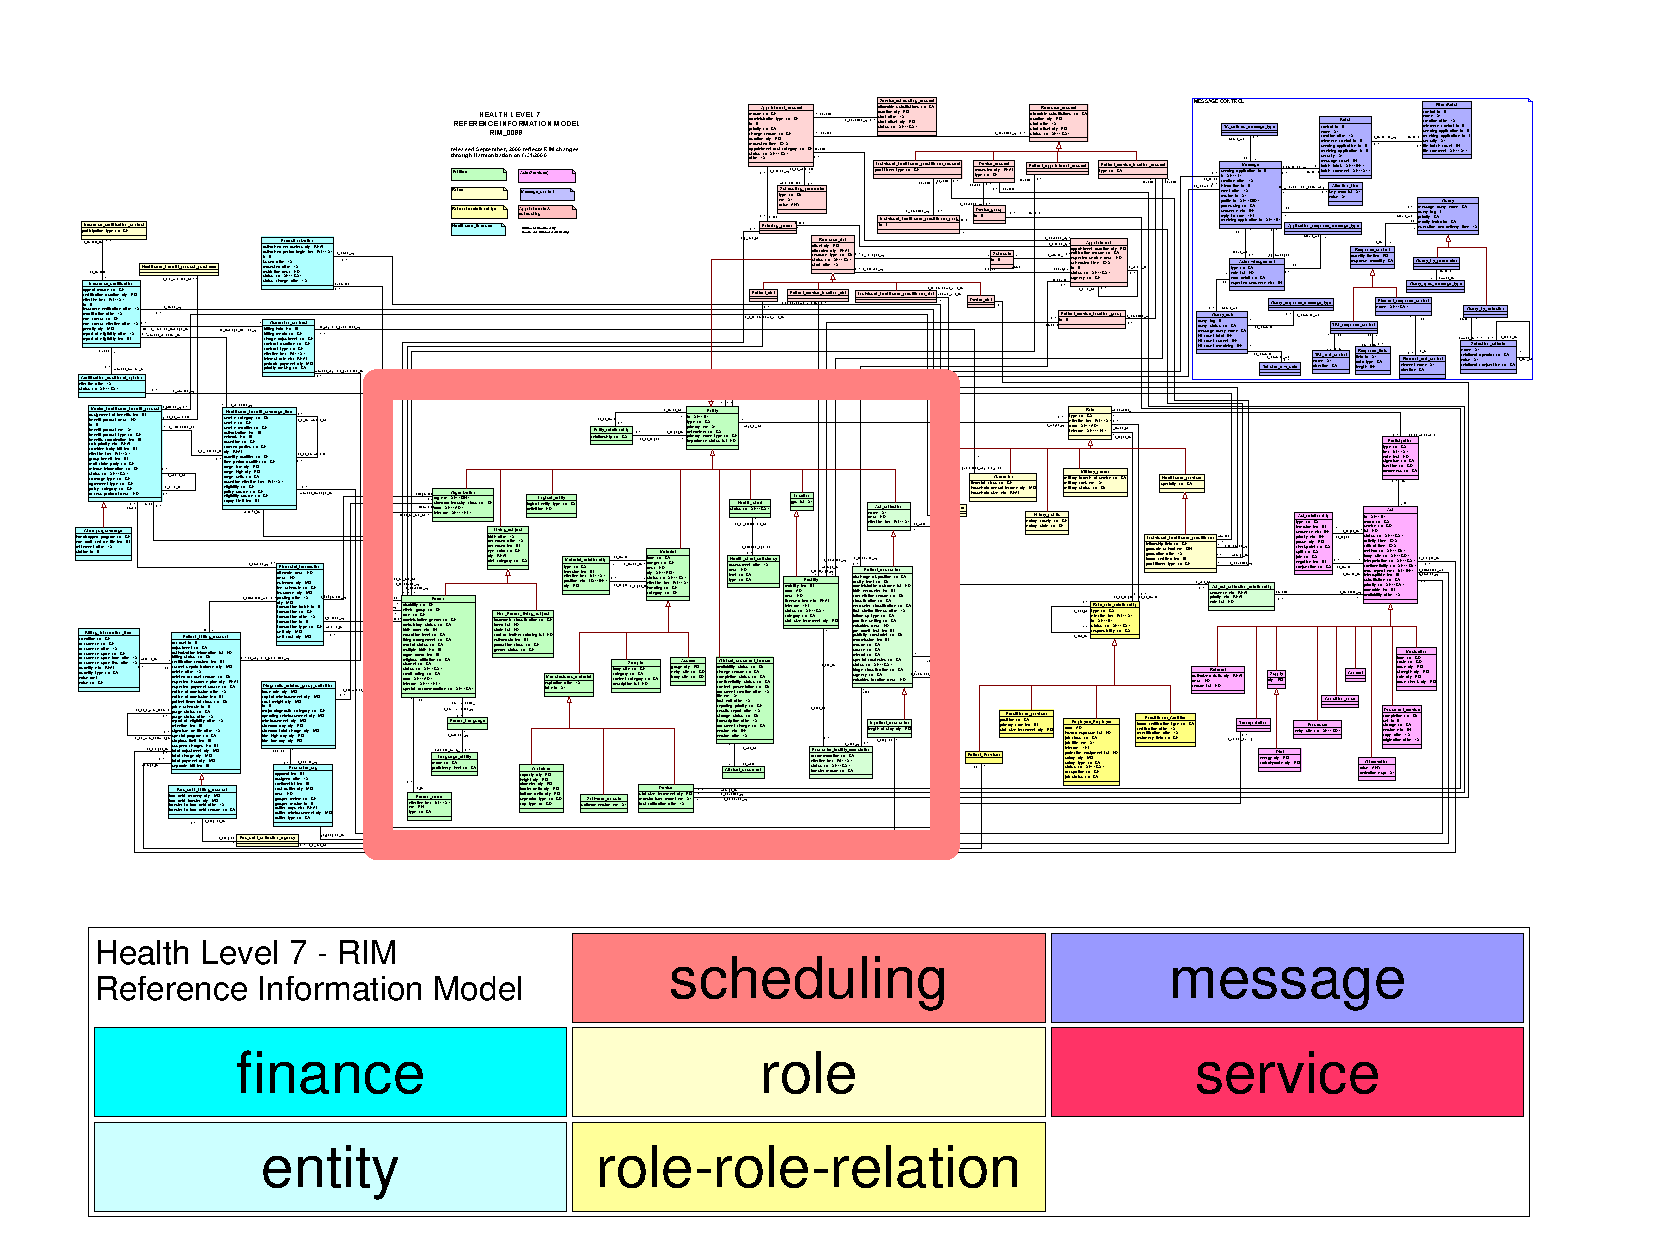
\includegraphics[scale=0.3,angle=-90]{graphic/rim.pdf}
        \caption{HL7 Reference Information Model Framework \cite{hl7}}
        \label{rim_figure}
    \end{center}
\end{figure}

\begin{figure}[ht]
    \begin{center}
        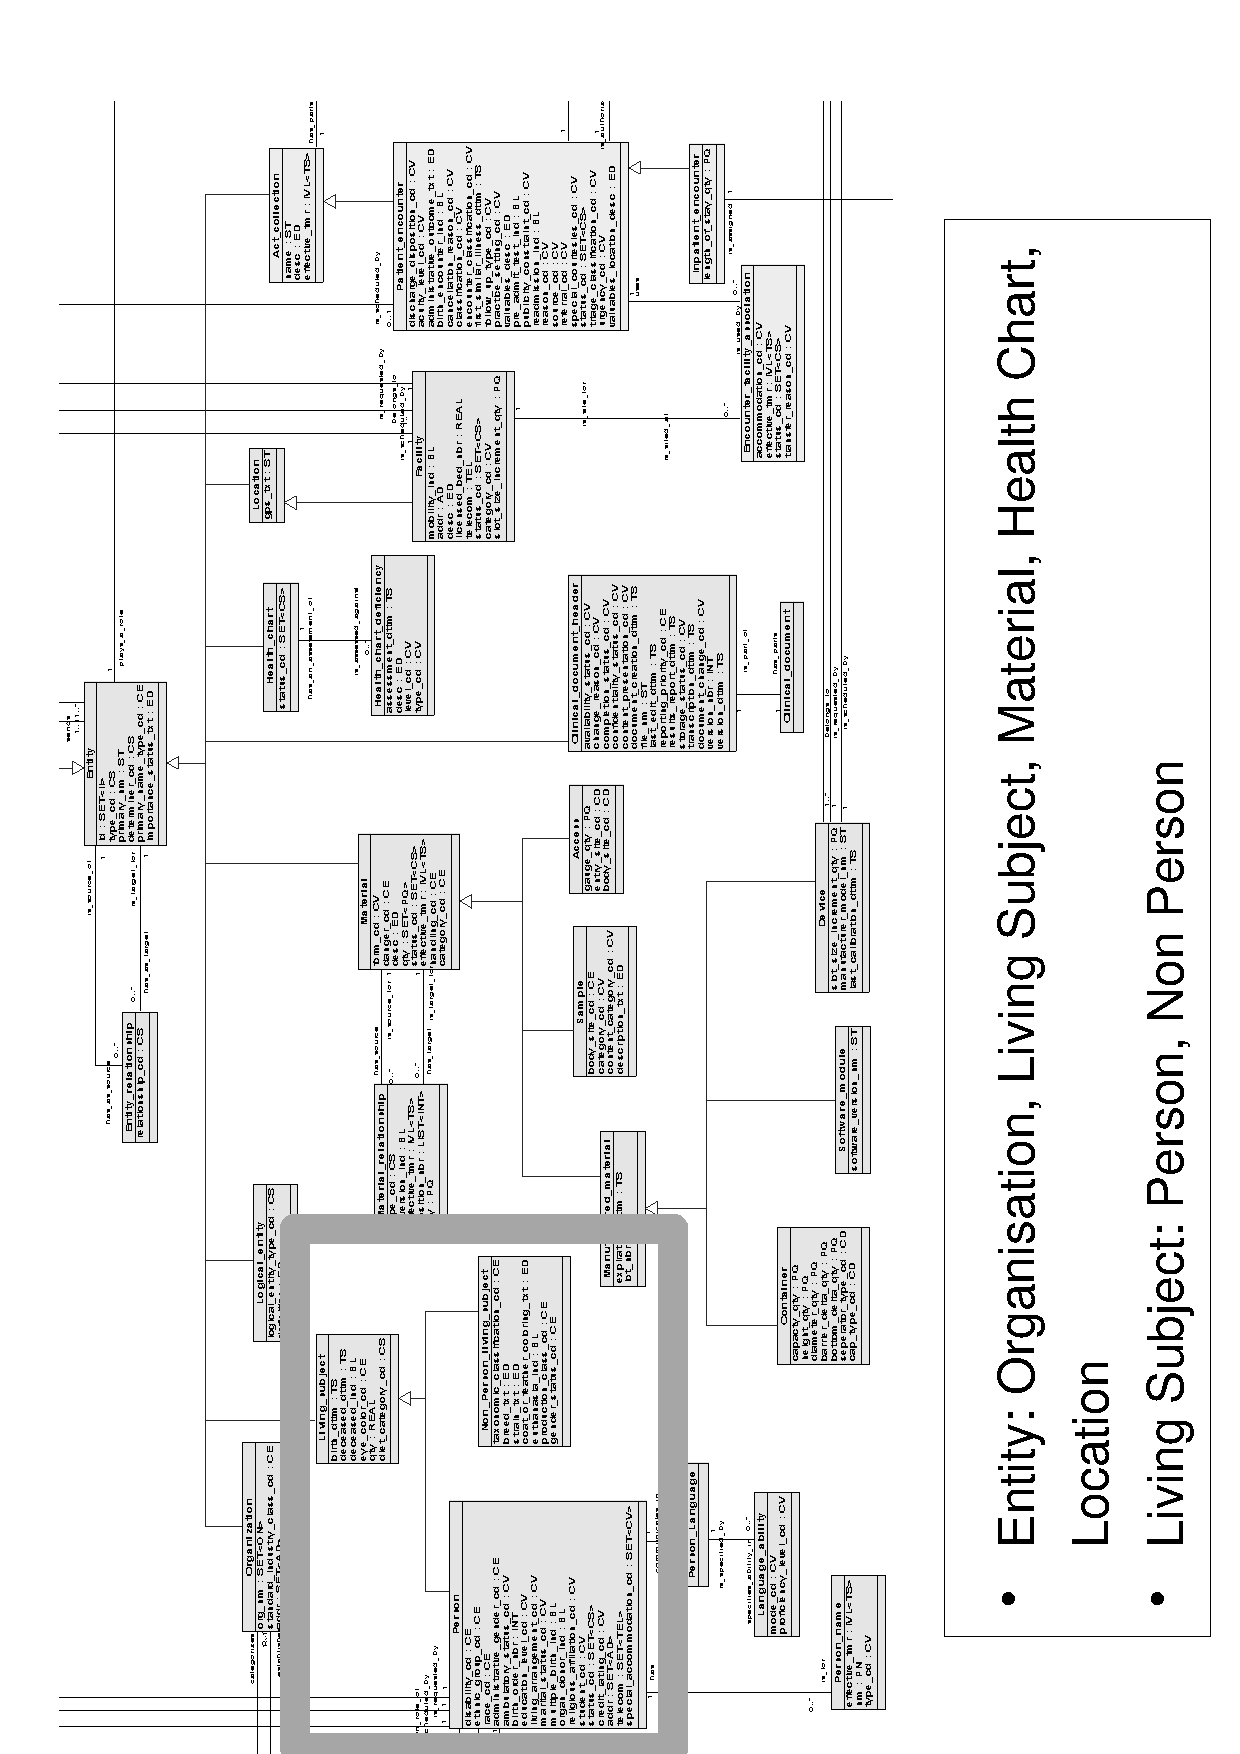
\includegraphics[scale=0.3,angle=-90]{graphic/entity.pdf}
        \caption{RIM Entities \cite{hl7}}
        \label{entity_figure}
    \end{center}
\end{figure}

\clearpage

If the RIM got implemented in the Java programming language, all of its classes
would inherit from the top-most super class \emph{java.lang.Object}. For reasons
of clearity, figure \ref{person_figure} omits several intermediary classes and
lets \emph{Living Subject} inherit directly from \emph{java.lang.Object}.

\begin{figure}[ht]
    \begin{center}
        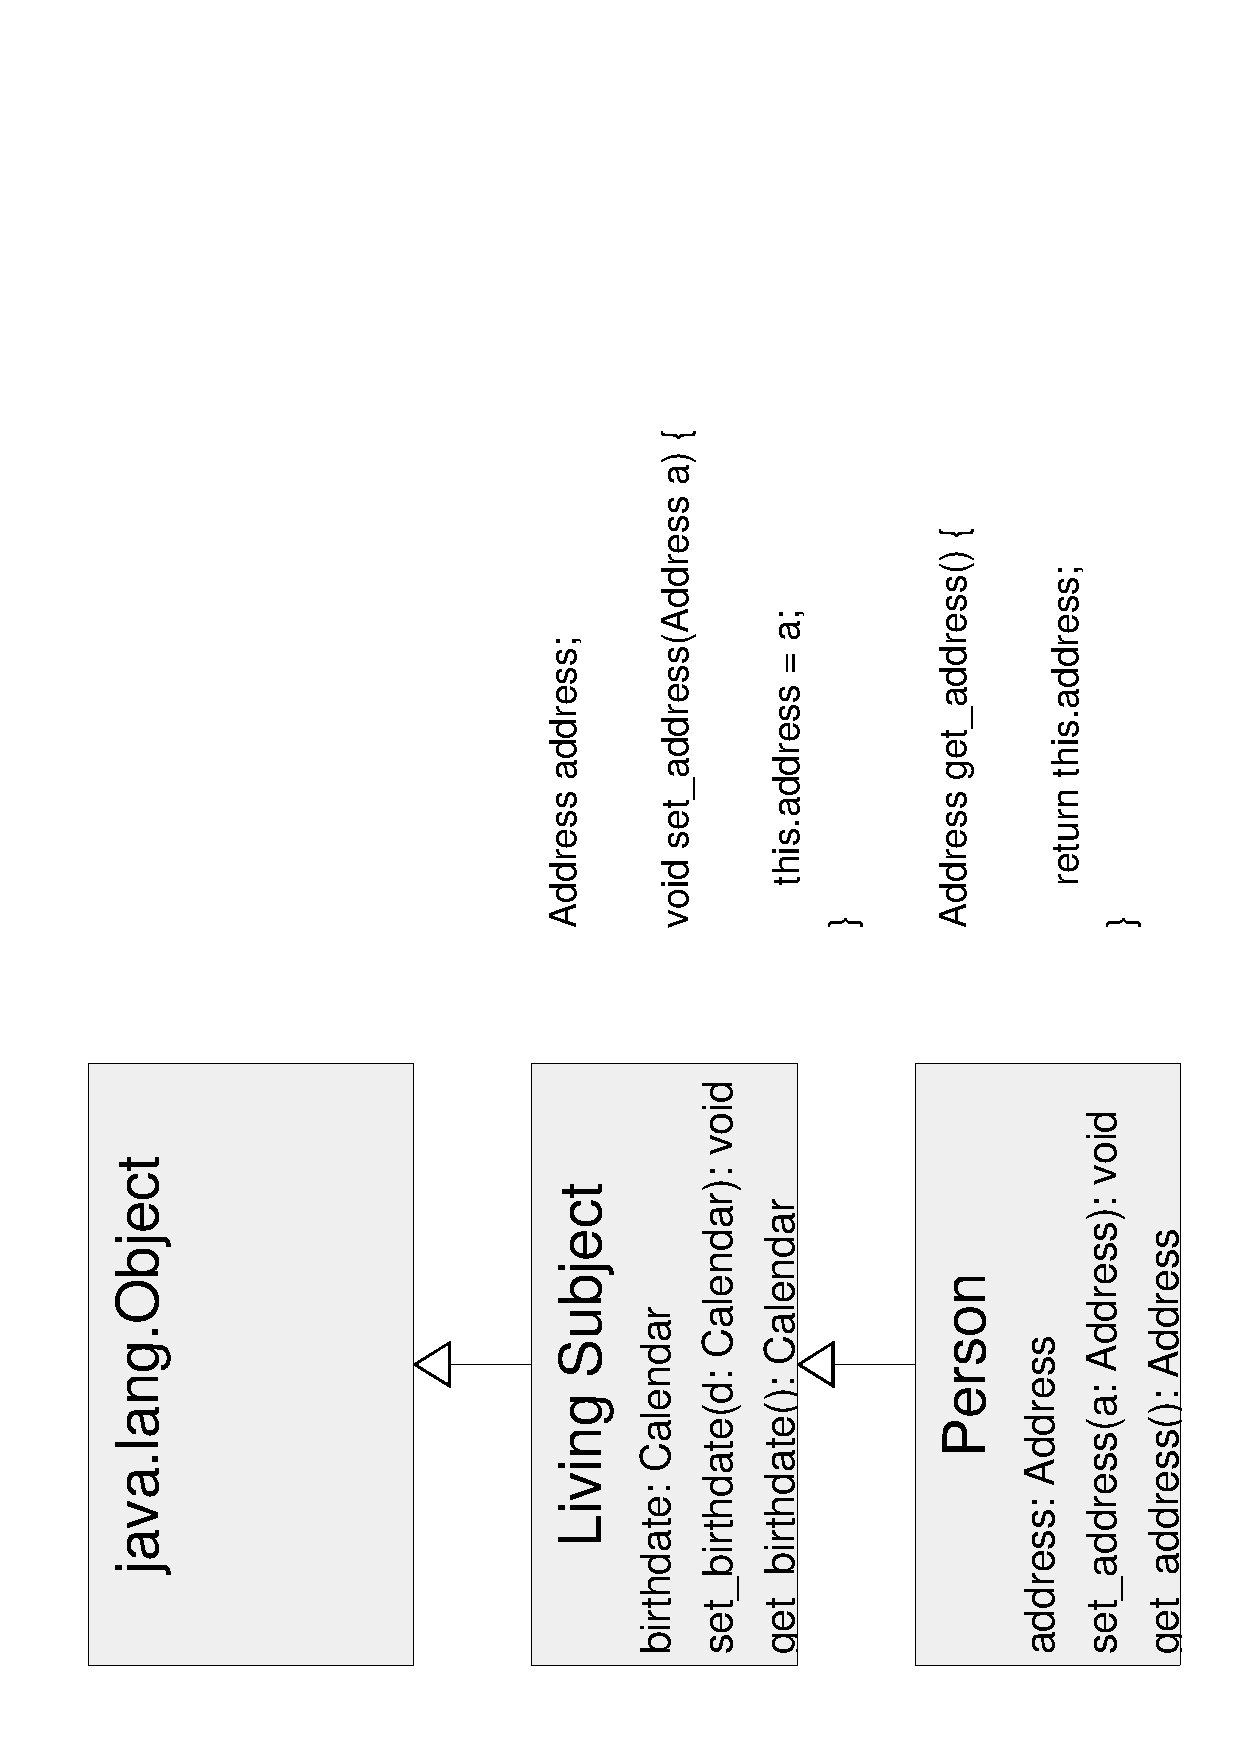
\includegraphics[scale=0.3,angle=-90]{graphic/person.pdf}
        \caption{Accessing a Person's Attributes}
        \label{person_figure}
    \end{center}
\end{figure}

Section \ref{association_elimination_heading} proposed to make the top-most
model in a tree of models inheriting from each other a \emph{Container}. In the
case of Java that would mean to add a container attribute such as one of type
\emph{HashMap}, together with the necessary access methods \emph{set},
\emph{get} and \emph{remove}, to the \emph{java.lang.Object} class (figure
\ref{hashmap_figure}).

That way, every abstract model (OO class) would, by default, become a container
able to store a hierarchy of sub models (objects). This would be much closer to
what section \ref{human_thinking_heading} worked out on the importance of the
principle of \emph{Composition} in human thinking, which perceives its
environment in form of discrete, but composed items. Every item in universe can
be seen as \emph{Compound} of yet smaller items. The basis of every modelling
effort must therefore be a \emph{Container Structure}.

This would also be a solution to the criticism of chapter
\ref{extended_motivation_heading}, meaning that: \textit{the hierarchy as
concept is not inherent in the type system of current programming languages}.

Additionally, access methods of classes inheriting from \emph{java.lang.Object}
(that is of \emph{all} classes) would become superfluous. Because every class
is a sub model of \emph{java.lang.Object}, every class can use not only its
container, but also the corresponding \emph{set}, \emph{get}, \emph{remove}
methods.

\begin{figure}[ht]
    \begin{center}
        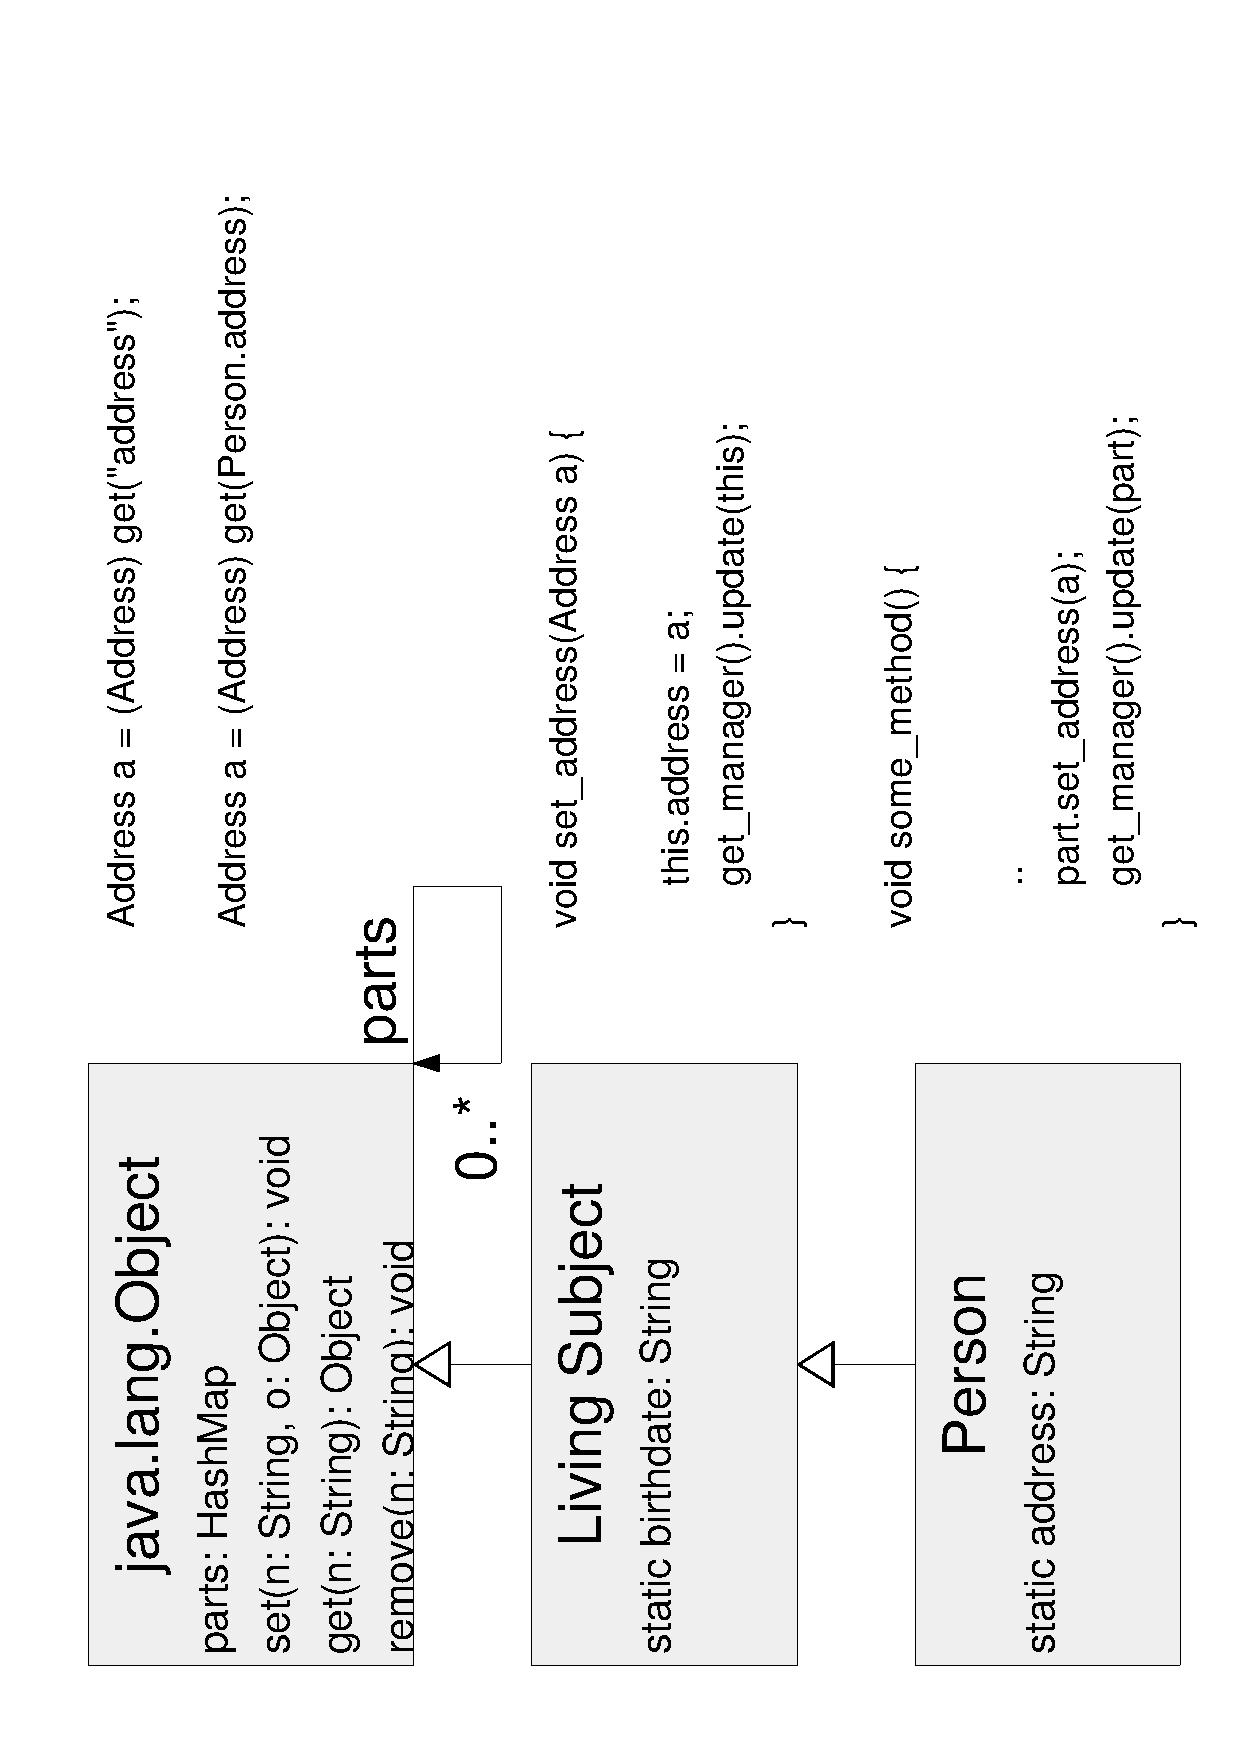
\includegraphics[scale=0.3,angle=-90]{graphic/hashmap.pdf}
        \caption{Access Method Elimination through Top-Level Container}
        \label{hashmap_figure}
    \end{center}
\end{figure}

On its top right-hand corner, figure \ref{hashmap_figure} shows the program code
that could be used to access an \emph{Address} as a \emph{Person}'s sub model.
In order to correctly identify the various attributes of a person, each of them
needs to carry a unique name. In the example of figure \ref{hashmap_figure},
the names are hold as static attributes of the classes they conceptually belong
to. But they can as well be stored somewhere else -- even in an external
configuration file, better called \emph{Knowledge Specification}.

One objection to the elimination of access methods in sub models could be that
then, necessary updates cannot be initiated. Traditionally, such updates are
often placed in the access methods directly. Figure \ref{hashmap_figure} shows
how an update manager is called in the \emph{set\_address} method, after the
\emph{address} attribute has been changed. However, the same update call can be
made outside the access method. It would possibly have to be called at several
places then, but judging from this work's author's experience with frameworks,
the number of update calls won't be too high and is usually well manageable.
The questionableness of the OO principle of \emph{Encapsulation} in general was
already mentioned in section \ref{encapsulation_heading}. Finally, there is
actually no access method-related code that cannot be handled alternatively.

%
% $RCSfile: categorisation_versus_composition.tex,v $
%
% Copyright (C) 2002-2008. Christian Heller.
%
% Permission is granted to copy, distribute and/or modify this document
% under the terms of the GNU Free Documentation License, Version 1.1 or
% any later version published by the Free Software Foundation; with no
% Invariant Sections, with no Front-Cover Texts and with no Back-Cover
% Texts. A copy of the license is included in the section entitled
% "GNU Free Documentation License".
%
% http://www.cybop.net
% - Cybernetics Oriented Programming -
%
% http://www.resmedicinae.org
% - Information in Medicine -
%
% Version: $Revision: 1.1 $ $Date: 2008-08-19 20:41:05 $ $Author: christian $
% Authors: Christian Heller <christian.heller@tuxtax.de>
%

\subsection{Categorisation versus Composition}
\label{categorisation_versus_composition_heading}
\index{Categorisation versus Composition}
\index{Object Oriented Programming}
\index{OOP}
\index{Fragile Base Class Problem}
\index{Misuse of Inheritance}
\index{Granularity}

Since the beginnings of \emph{Object Oriented Programming} (OOP), several of
its paradigms were reflected critically and found to cause problems. One of
them is the \emph{Fragile Base Class Problem} explained in section
\ref{fragile_base_class_heading}.

\begin{figure}[ht]
    \begin{center}
        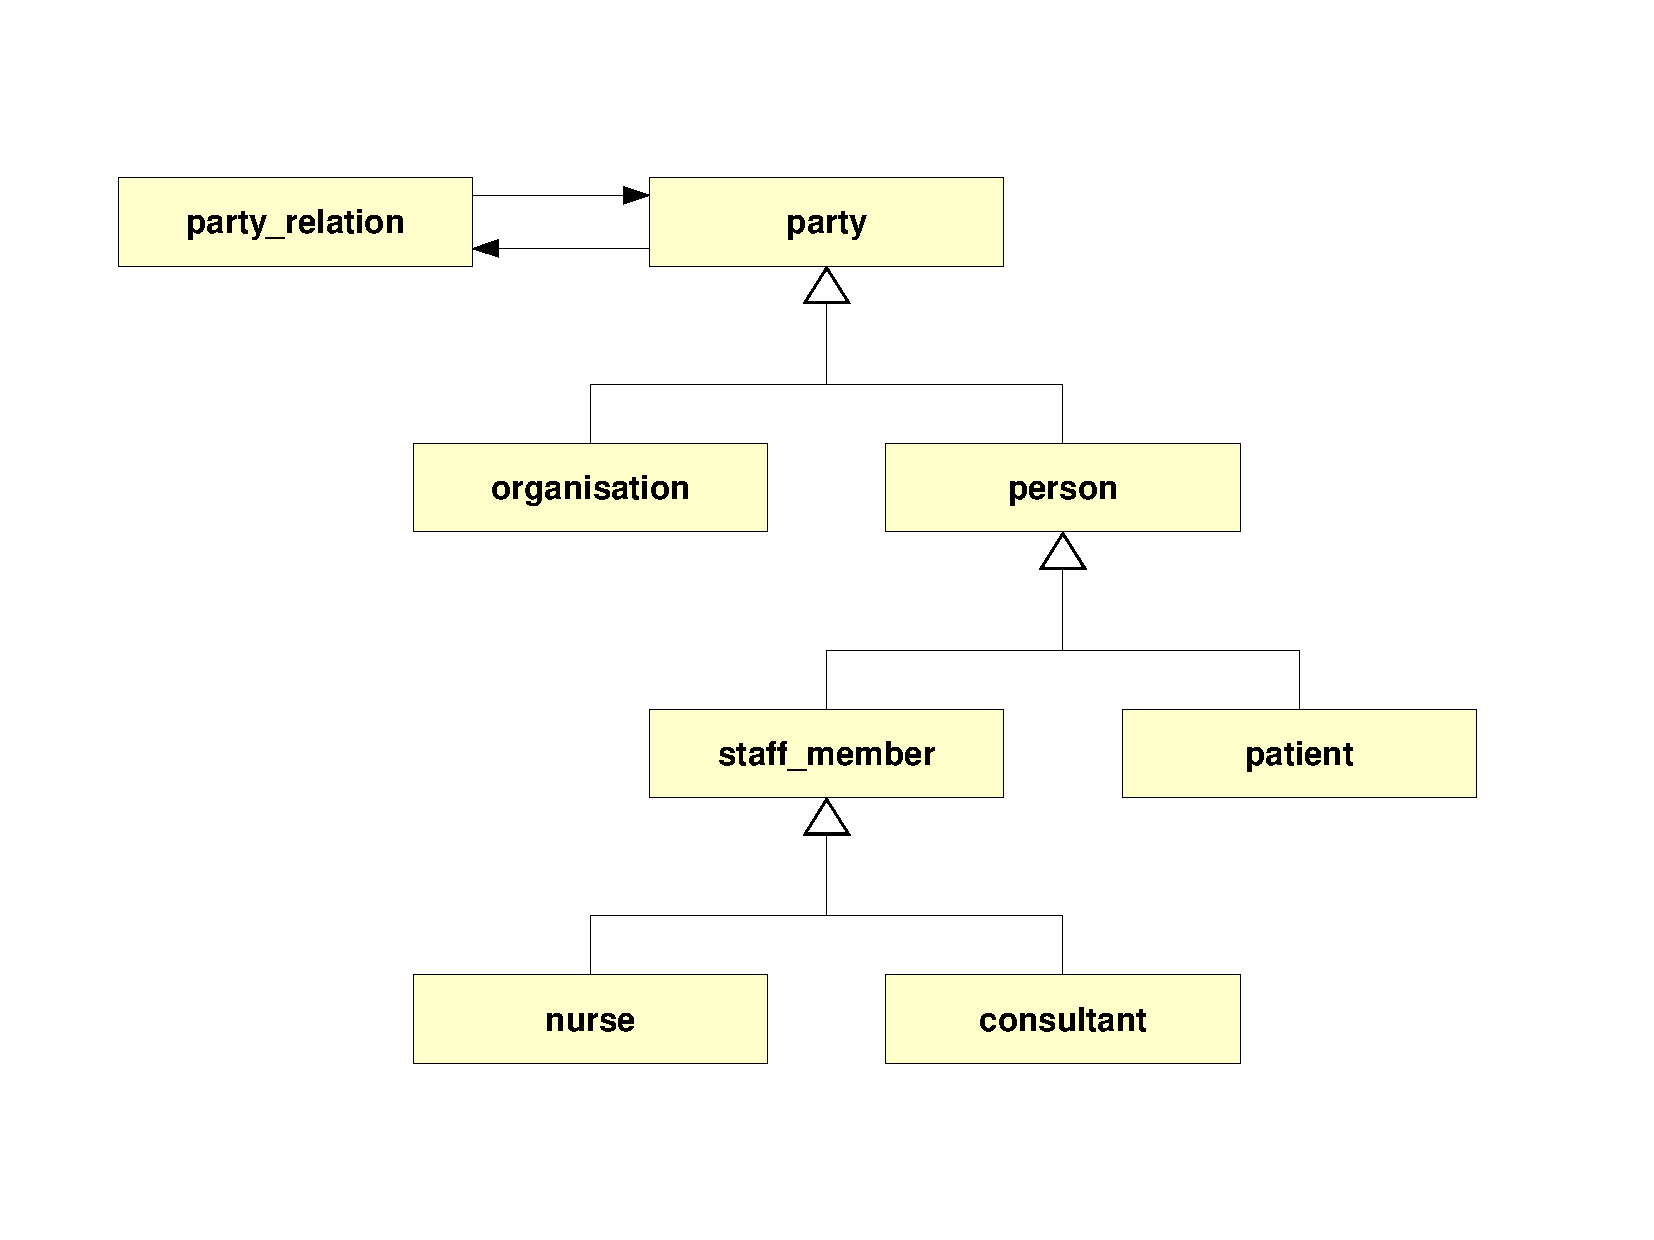
\includegraphics[scale=0.3,angle=-90]{graphic/party.pdf}
        \caption{Categorisation versus Composition of Parties \cite[p. 12]{archetypes}}
        \label{party_figure}
    \end{center}
\end{figure}

Further problems may occur through the misuse of inheritance, leading to bad
design solutions. A typical example is the modelling of demographic entities
like \emph{Patient} or \emph{Nurse} as subtypes of \emph{Person} (figure
\ref{party_figure}), whilst actually, they are \emph{Party Relationships}
\cite[p. 12]{archetypes}, \cite{fowler1997}.

As can be seen, inheritance can create more problems than are foreseeable. One
way to circumvent unwanted dependencies is to sort abstract models according to
their placement within a larger model surrounding them. Part models of a model
may be grouped by their level of \emph{Granularity}. It should never be only
\emph{Properties} leading to the creation of a super category.

A main reason for using inheritance is the reuse of functionality in form of
methods. If methods as logic models were kept externally of state models,
inheritance as way to reuse methods would not be necessary anymore (section
\ref{state_and_logic_heading}).

% ?? %
% $RCSfile: archetype.tex,v $
%
% Copyright (C) 2002-2008. Christian Heller.
%
% Permission is granted to copy, distribute and/or modify this document
% under the terms of the GNU Free Documentation License, Version 1.1 or
% any later version published by the Free Software Foundation; with no
% Invariant Sections, with no Front-Cover Texts and with no Back-Cover
% Texts. A copy of the license is included in the section entitled
% "GNU Free Documentation License".
%
% http://www.cybop.net
% - Cybernetics Oriented Programming -
%
% http://www.resmedicinae.org
% - Information in Medicine -
%
% Version: $Revision: 1.1 $ $Date: 2008-08-19 20:41:05 $ $Author: christian $
% Authors: Christian Heller <christian.heller@tuxtax.de>
%

\subsection{Archetype}
\label{archetype_heading}
\index{Archetype}
\index{Electronic Health Record}
\index{EHR}
\index{Good European/ EHR}
\index{GEHR}
\index{Open EHR}
\index{SNOMED CT}
\index{Archetype Definition Language}
\index{ADL}
\index{Constraint Form of ADL}
\index{cADL}
\index{Data Definition Form of ADL}
\index{dADL}
\index{Template Form of ADL}
\index{tADL}
\index{First Order Predicate Logic}
\index{FOPL}

With the aim of providing the means to build usable, maintainable, extensible
\emph{Electronic Health Records} (EHR), the \emph{Archetype} as design concept
was introduced in the \emph{Design Principles} document of the
\emph{Good European/ EHR} (GEHR) project, which was later renamed into
\emph{Open EHR} \cite{openehr}. Their website states: \textit{An archetype is a
re-usable, formal model of a domain concept.} Archetypes adhere to ontological
principles; they can be composed of other archetypes or atomic elements. Their
use is not limited to EHR building, despite OpenEHR's focus on the medical
domain.

Comparing archetypes with terminologies, Beale \cite{openehrtechnical} writes
that a terminology like for example SNOMED Clinical Terms (SNOMED CT) had the
form of a semantic network, i.e. \ldots\ with an ontological flavour. However,
because rigorous design principles were not always applied, they tended to be
internally inconsistent and had a lot of pre-coordination in them, while what
was really needed was a generative/ compositional terminology. Further, SNOMED
could tell what the meanings of the parts of e.g. a complete blood count test
are, but it were not going to provide a model of an actual blood test. This is
where archetypes \ldots\ would come in; they were about information
\emph{in use}, not definitions of reality (as terminologies). \ldots\ So --
even if SNOMED was perfect, it wouldn't do everything. It were a knowledge
support part of the environment, and it could be used to name things and
perform inferencing (\textit{draw a conclusion/ deduction} \cite{websters}).

An \emph{Archetype Definition Language} (ADL) \cite{adl} was created for the
specification of archetypes. A corresponding ADL document has the following
structure:

\begin{scriptsize}
    \begin{verbatim}
    archetype_id = <"some.archetype.id">
    adl_version = <"2.0">
    is_controlled = <True>
    parent_archetype_id = <"some.other.archetype.id">
    concept = <[concept_code]>
    original_language = <"lang">
    translations = <
    ...
    >
    description = <
    ...
    >
    definition = <
    cADL structural section
    >
    invariant = <
    assertions
    >
    ontology = <
    ...
    >
    revision_history = <
    ...
    >
    \end{verbatim}
\end{scriptsize}

Many separate sections can be identified in this archetype structure, and
various syntaxes are used for them. Table \ref{adl_table} gives an overview of
the structural elements of an ADL archetype. In addition to the single
sections, it mentions two further syntaxes, for templates and constraints on
data instances.

\begin{table}[ht]
    \begin{center}
        \begin{footnotesize}
        \begin{tabular}{| p{30mm} | p{30mm} | p{45mm} |}
            \hline
            \textbf{Element} & \textbf{Syntax} & \textbf{Purpose}\\
            \hline
            archetype structure & \emph{Archetype Definition Language} (ADL) & glue syntax\\
            \hline
            definition section & \emph{Constraint Form of ADL} (cADL) &
                constraints definition\\
            \hline
            description, ontology and other sections & \emph{Data Definition Form of ADL} (dADL) &
                data definition\\
            \hline
            template & \emph{Template Form of ADL} (tADL) &
                formalism to compose archetypes into larger constraint structures, used in particular contexts at runtime\\
            \hline
            data instances & \emph{First Order Predicate Logic} (FOPL) &
                constraints on data which are instances of some information model (e.g. expressed in UML)\\
            \hline
        \end{tabular}
        \end{footnotesize}
        \caption{Structural Elements of an ADL-defined Archetype \cite{adl}}
        \label{adl_table}
    \end{center}
\end{table}

Chapter \ref{cybernetics_oriented_language_heading} will define a new language
that is based on just one syntax: the \emph{Extensible Markup Language} (XML)
(section \ref{extensible_markup_language_heading}), an easy-to-grasp pure text
format. Despite its limited vocabulary of just four tags and four attributes,
that language may encode a rich set of knowledge constructs, including meta
information and constraints.
 ALREADY input by "conceptual_network"!

%
% $RCSfile: knowledge_representation.tex,v $
%
% Copyright (C) 2002-2008. Christian Heller.
%
% Permission is granted to copy, distribute and/or modify this document
% under the terms of the GNU Free Documentation License, Version 1.1 or
% any later version published by the Free Software Foundation; with no
% Invariant Sections, with no Front-Cover Texts and with no Back-Cover
% Texts. A copy of the license is included in the section entitled
% "GNU Free Documentation License".
%
% http://www.cybop.net
% - Cybernetics Oriented Programming -
%
% http://www.resmedicinae.org
% - Information in Medicine -
%
% Version: $Revision: 1.1 $ $Date: 2008-08-19 20:41:07 $ $Author: christian $
% Authors: Christian Heller <christian.heller@tuxtax.de>
%

\section{Knowledge Representation}
\label{knowledge_representation_heading}
\index{Knowledge Representation}

Section \ref{human_thinking_heading} identified the abstraction principles of
human thinking, before section \ref{design_reflections_heading} reflected on
their impact on software design. The final considerations of this chapter now
deal with a possible architecture for knowledge representation (as first
presented in \cite{heller2006}), which applies the principles of human thinking.

%
% $RCSfile: knowledge_ontology.tex,v $
%
% Copyright (C) 2002-2008. Christian Heller.
%
% Permission is granted to copy, distribute and/or modify this document
% under the terms of the GNU Free Documentation License, Version 1.1 or
% any later version published by the Free Software Foundation; with no
% Invariant Sections, with no Front-Cover Texts and with no Back-Cover
% Texts. A copy of the license is included in the section entitled
% "GNU Free Documentation License".
%
% http://www.cybop.net
% - Cybernetics Oriented Programming -
%
% http://www.resmedicinae.org
% - Information in Medicine -
%
% Version: $Revision: 1.1 $ $Date: 2008-08-19 20:41:07 $ $Author: christian $
% Authors: Christian Heller <christian.heller@tuxtax.de>
%

\subsection{Knowledge Ontology}
\label{knowledge_ontology_heading}
\index{Knowledge Ontology}
\index{Composition}
\index{Ontology}
\index{Ontological Level}
\index{Granularity}

The previous sections tried to demonstrate the importance of \emph{Composition}
for knowledge modelling. One technique that was mentioned in this context are
\emph{Ontologies}. Section \ref{conceptual_network_heading} introduced some of
its numerous definitions. Section \ref{association_elimination_heading}
demonstrated how the principle of \emph{Hierarchy} may be applied to obtain an
\emph{Ontology}. The layers forming an ontology were called
\emph{Ontological Level}.

Basically, an ontology represents a systematic description of complex domain
contexts. This work uses its own adapted definition, and considers an ontology
to be \emph{a strict hierarchy of abstract models, organised in levels of
growing granularity, that are solely unidirectionally related}.

Terminologies as described in section \ref{terminology_heading} may be used to
specify the basic elements of an ontology. Every term may be represented by an
own abstract model (concept) containing a number of strings, one for each
terminology system. Further strings may stand for language translations, which
has importance for \emph{Internationalisation}.

The following examples may seem simple, but want to strengthen the hierarchical
thinking of the reader, under consideration of the granularity of models.

%
% $RCSfile: biological_systems.tex,v $
%
% Copyright (C) 2002-2008. Christian Heller.
%
% Permission is granted to copy, distribute and/or modify this document
% under the terms of the GNU Free Documentation License, Version 1.1 or
% any later version published by the Free Software Foundation; with no
% Invariant Sections, with no Front-Cover Texts and with no Back-Cover
% Texts. A copy of the license is included in the section entitled
% "GNU Free Documentation License".
%
% http://www.cybop.net
% - Cybernetics Oriented Programming -
%
% http://www.resmedicinae.org
% - Information in Medicine -
%
% Version: $Revision: 1.1 $ $Date: 2008-08-19 20:41:05 $ $Author: christian $
% Authors: Christian Heller <christian.heller@tuxtax.de>
%

\subsubsection{Biological Systems}
\label{biological_systems_heading}
\index{Biological System as Ontology}
\index{Ontological Layer}
\index{Parallel Layer}
\index{Stratum}

One example showing the hierarchical structuring of biological systems is
mentioned in \cite{sengbusch}. Its models are listed in decreasing granularity,
in table \ref{biological_table}.

\begin{table}[ht]
    \begin{center}
        \begin{footnotesize}
        \begin{tabular}{| p{105mm} |}
            \hline
            \textbf{Biological System}\\
            \hline
            Ecosystem\\
            \hline
            Biocoenosis (Living Community)\\
            \hline
            Multiple Cell Organism\\
            \hline
            Single Cell Organism (Protozoa)\\
            \hline
            Organelle (Mitochondrie, Chloroplast)\\
            \hline
            Supra Molecular Complex (Ribosome, Chromosome, Membrane)\\
            \hline
            Small Molecule\\
            \hline
        \end{tabular}
        \end{footnotesize}
        \caption{Hierarchical Structuring of Biological Systems}
        \label{biological_table}
    \end{center}
\end{table}

It is important not to mix ontological layers with parallel layers. In
\emph{Geology} or \emph{Biology}, the latter (also called \emph{Stratum}) may
be layers of material arranged one on top of another (such as a layer of tissue
or cells in an organism) \cite{wordnet}. However, these are not \emph{composed}
of each other. Ontological layers, on the other hand, have a different level of
granularity, each so that higher-level abstractions are composed of lower-level
abstractions.

%
% $RCSfile: logical_book.tex,v $
%
% Copyright (C) 2002-2008. Christian Heller.
%
% Permission is granted to copy, distribute and/or modify this document
% under the terms of the GNU Free Documentation License, Version 1.1 or
% any later version published by the Free Software Foundation; with no
% Invariant Sections, with no Front-Cover Texts and with no Back-Cover
% Texts. A copy of the license is included in the section entitled
% "GNU Free Documentation License".
%
% http://www.cybop.net
% - Cybernetics Oriented Programming -
%
% http://www.resmedicinae.org
% - Information in Medicine -
%
% Version: $Revision: 1.1 $ $Date: 2008-08-19 20:41:07 $ $Author: christian $
% Authors: Christian Heller <christian.heller@tuxtax.de>
%

\subsubsection{Logical Book}
\label{logical_book_heading}
\index{Logical Book as Ontology}
\index{Extension of Ontologies}
\index{Physical Book as Ontology}

The logical structure of a \emph{Book} shall serve as second example. A
\emph{Chapter} may consist of \emph{Paragraphs}. Yet it may become necessary to
first subdivide \emph{Chapter} into \emph{Sections} which then consist of
\emph{Paragraphs}, as shown in table \ref{book_table}.

All ontologies can get extended \emph{up-} or \emph{downwards}, by adding
further levels, at any later point in design time. But they can as well get
extended by inserting \emph{Intermediate Layers} between two already existing
ones. However, additional levels should only get introduced if there really is
a need for them.

\begin{table}[ht]
    \begin{center}
        \begin{footnotesize}
        \begin{tabular}{| p{105mm} |}
            \hline
            \textbf{Model Category}\\
            \hline
            Library\\
            \hline
            Book\\
            \hline
            Part\\
            \hline
            Chapter\\
            \hline
            Section\\
            \hline
            Paragraph\\
            \hline
            Sentence\\
            \hline
            Word\\
            \hline
            Character\\
            \hline
        \end{tabular}
        \end{footnotesize}
        \caption{Logical Book}
        \label{book_table}
    \end{center}
\end{table}

In contrast to the division of a \emph{logical} book, a \emph{physical} book
may be structured completely differently, for example into \emph{Binding},
\emph{Cover} and \emph{Pages}. Of course, the contents of an ontology heavily
depends on the intended area of application (knowledge domain) of the software
to be created.

%
% $RCSfile: interdisciplinary_science.tex,v $
%
% Copyright (C) 2002-2008. Christian Heller.
%
% Permission is granted to copy, distribute and/or modify this document
% under the terms of the GNU Free Documentation License, Version 1.1 or
% any later version published by the Free Software Foundation; with no
% Invariant Sections, with no Front-Cover Texts and with no Back-Cover
% Texts. A copy of the license is included in the section entitled
% "GNU Free Documentation License".
%
% http://www.cybop.net
% - Cybernetics Oriented Programming -
%
% http://www.resmedicinae.org
% - Information in Medicine -
%
% Version: $Revision: 1.1 $ $Date: 2008-08-19 20:41:07 $ $Author: christian $
% Authors: Christian Heller <christian.heller@tuxtax.de>
%

\subsubsection{Interdisciplinary Science}
\label{interdisciplinary_science_heading}
\index{Interdisciplinary Science}
\index{System of Sciences}
\index{Sciences as Ontology}
\index{Cybernetics}

A third, certainly very subjective example tries to sort a number of known
\emph{Sciences} into one common system (table \ref{sciences_table}).
\emph{Arts}, \emph{Linguistics}, \emph{Mathematics} and \emph{Informatics} have
an extra status: They deal with already abstracted knowledge (paintings, music,
language, numbers) and can be used as utility by any of the other sciences.

\begin{table}[ht]
    \begin{center}
        \begin{footnotesize}
        \begin{tabular}{| p{35mm} | p{70mm} |}
            \hline
            \textbf{Scientific Subject} & \textbf{Example Model}\\
            \hline
            Astronomy & Celestial Body (Big Bang, Cosmos)\\
            \hline
            Biology & Living Thing (Human, Animal, Plant, Virus)\\
            \hline
            Geography & Dead Thing (Air, Fire, Stone, Crystal)\\
            \hline
            Chemistry & Compounds (Water, DNA)\\
            \hline
            Physics & Particles (Elementary Particle, Atom, Matter, Energy)\\
            \hline
            Philosophy / Religion & Dialectic Dualism (Matter/Anti-Matter, +/-, 0/1)\\
            \hline
        \end{tabular}
        \end{footnotesize}
        \caption{System of Sciences}
        \label{sciences_table}
    \end{center}
\end{table}

The whole effort of finding new ways for representing knowledge, as done in
this work, is an \emph{inter-disciplinary} undertaking itself, touching various
fields of science. The world (nature) needs to be understood in its basics so
that humans are enabled to copy its concepts and put them into artificial
models -- exactly what \emph{Cybernetics} is all about.

%
% $RCSfile: car_model.tex,v $
%
% Copyright (C) 2002-2008. Christian Heller.
%
% Permission is granted to copy, distribute and/or modify this document
% under the terms of the GNU Free Documentation License, Version 1.1 or
% any later version published by the Free Software Foundation; with no
% Invariant Sections, with no Front-Cover Texts and with no Back-Cover
% Texts. A copy of the license is included in the section entitled
% "GNU Free Documentation License".
%
% http://www.cybop.net
% - Cybernetics Oriented Programming -
%
% http://www.resmedicinae.org
% - Information in Medicine -
%
% Version: $Revision: 1.1 $ $Date: 2008-08-19 20:41:05 $ $Author: christian $
% Authors: Christian Heller <christian.heller@tuxtax.de>
%

\subsubsection{Car Model}
\label{car_model_heading}
\index{Car Model as Ontology}
\index{Computer Aided Design}
\index{CAD}
\index{Computer Aided Manufacturing}
\index{CAM}
\index{Unidirectional Relation}
\index{Layers of an Abstract Model}
\index{Levels of an Abstract Model}

A \emph{Computer Aided Design} (CAD)/ \emph{Computer Aided Manufacturing} (CAM)
system of a car manufacturer will have a \emph{Car} model like the one shown in
table \ref{car_table}.

\begin{table}[ht]
    \begin{center}
        \begin{footnotesize}
        \begin{tabular}{| p{105mm} |}
            \hline
            \textbf{Model Category}\\
            \hline
            Car\\
            \hline
            Body, Chassis, Engine, Transmission\\
            \hline
            Door, Axle, Wheel, Cylinder\\
            \hline
            Window, Suspension, Plunger\\
            \hline
        \end{tabular}
        \end{footnotesize}
        \caption{Car Model}
        \label{car_table}
    \end{center}
\end{table}

The ontology contains multiple categories of models which are composed of each
other. An \emph{Engine} consists of a \emph{Cylinder} which consists of a
\emph{Plunger} and so on. That is why people speak of different \emph{Layers}
or \emph{Levels} of abstract models. An \emph{Axle} belongs to one level and a
\emph{Chassis} belongs to another, higher level. In a good ontology, the
relations between models are always \emph{unidirectional}, that is a chassis
can link to axles but not the other way.

%
% $RCSfile: macrocosm_and_microcosm.tex,v $
%
% Copyright (C) 2002-2008. Christian Heller.
%
% Permission is granted to copy, distribute and/or modify this document
% under the terms of the GNU Free Documentation License, Version 1.1 or
% any later version published by the Free Software Foundation; with no
% Invariant Sections, with no Front-Cover Texts and with no Back-Cover
% Texts. A copy of the license is included in the section entitled
% "GNU Free Documentation License".
%
% http://www.cybop.net
% - Cybernetics Oriented Programming -
%
% http://www.resmedicinae.org
% - Information in Medicine -
%
% Version: $Revision: 1.1 $ $Date: 2008-08-19 20:41:07 $ $Author: christian $
% Authors: Christian Heller <christian.heller@tuxtax.de>
%

\subsubsection{Macrocosm and Microcosm}
\label{macrocosm_and_microcosm_heading}
\index{Macrocosm as Part of an Ontology}
\index{Microcosm as Part of an Ontology}
\index{Astronomical Particles as Ontology}
\index{Universe}
\index{Top Level Model}
\index{Concept}
\index{Electronic Health Record}
\index{EHR}
\index{Electronic Insurance Record}
\index{EIR}

Table \ref{astronomical_table} lists \emph{Astronomical Particles}
\cite{fernandezdavid, arnett}. It ends with the \emph{Universe} and an
undefinable \emph{Macrocosm}.

\begin{table}[ht]
    \begin{center}
        \begin{footnotesize}
        \begin{tabular}{| p{40mm} | p{65mm} |}
            \hline
            \textbf{Category} & \textbf{Example Model}\\
            \hline
            Macrocosm & (Infinity)\\
            \hline
            Universe & Our Universe with its Laws of Nature\\
            \hline
            Heap of Galaxies & Local Group, Heap of Virgo\\
            \hline
            Galaxy & Milky Way (our), Andromeda, Magellan's Clouds\\
            \hline
            Planetary (Solar) System & Sol (Sun), 51 Pegasi\\
            \hline
            Star/ Planet & Beta Pictoris, Mercury, Venus, Earth, Mars\\
            \hline
        \end{tabular}
        \end{footnotesize}
        \caption{Astronomical Particles}
        \label{astronomical_table}
    \end{center}
\end{table}

When trying to abstract things (in software), there has to be some limit, a
kind of \emph{Top Level Model}. It represents the \emph{Concept} to be
described. For a medical information system, one such top level model will be
the \emph{Electronic Health Record} (EHR); for an insurance application, it
will be the \emph{Electronic Insurance Record} (EIR); and so on.

Models do not only have to be limited \emph{upwards}; the same holds true for
modelling towards \emph{Microcosm}. Table \ref{physical_table} organises
particles, as used by natural sciences, into several categories.

\begin{table}[ht]
    \begin{center}
        \begin{footnotesize}
        \begin{tabular}{| p{50mm} | p{55mm} |}
            \hline
            \textbf{Category} & \textbf{Example Model}\\
            \hline
            Physical Compound & Air, Water, Fire, Ground\\
            \hline
            Chemical Compound/ Molecule & H$_{2}$, O$_{2}$, O$_{3}$, H$_{2}$O\\
            \hline
            Crystal & C (Diamond)\\
            \hline
            Atom (Chemical Element) & H, He, O\\
            \hline
            Elementary Particle & Quark, Lepton (Electron, Neutrino)\\
            \hline
            Urelement & (Primary Particle)\\
            \hline
            Microcosm & (Infinity)\\
            \hline
        \end{tabular}
        \end{footnotesize}
        \caption{Physical Particles}
        \label{physical_table}
    \end{center}
\end{table}

Although the real world seems to be built like that (infinite, nobody knowing
what comes beneath the \emph{Quark} particles) -- in software modelling it
makes no sense (and is actually impossible) to neverendingly introduce lower
and lower levels, towards \emph{Microcosm}. On some point, the hierarchy has to
be stopped, to be able to abstract it in software. The later chapter
\ref{state_and_logic_heading} gives an overview of common knowledge primitives.


%
% $RCSfile: schema.tex,v $
%
% Copyright (c) 2005-2006. Christian Heller. All rights reserved.
%
% Permission is granted to copy, distribute and/or modify this document
% under the terms of the GNU Free Documentation License, Version 1.1 or
% any later version published by the Free Software Foundation; with no
% Invariant Sections, with no Front-Cover Texts and with no Back-Cover
% Texts. A copy of the license is included in the section entitled
% "GNU Free Documentation License".
%
% http://www.cybop.net
% - Cybernetics Oriented Programming -
%
% http://www.resmedicinae.org
% - Information in Medicine -
%
% Version: $Revision: 1.1 $ $Date: 2006-01-03 08:21:45 $ $Author: christian $
% Authors: Christian Heller <christian.heller@tuxtax.de>
%

\subsubsection{Schema}
\label{schema_heading}

A theoretical \emph{Model} is an abstract clip of the real world, and exists in
the human mind. Another common word for \emph{Model} is \emph{Concept}. It is
the subsumption of \emph{Item}, \emph{Category} and \emph{Compound}, resulting
from three activities of abstraction: \emph{Discrimination},
\emph{Categorisation} and \emph{Composition} \cite{heller2004}. Each model
\emph{knows} about the parts it consists of.

\begin{figure}[ht]
    \begin{center}
        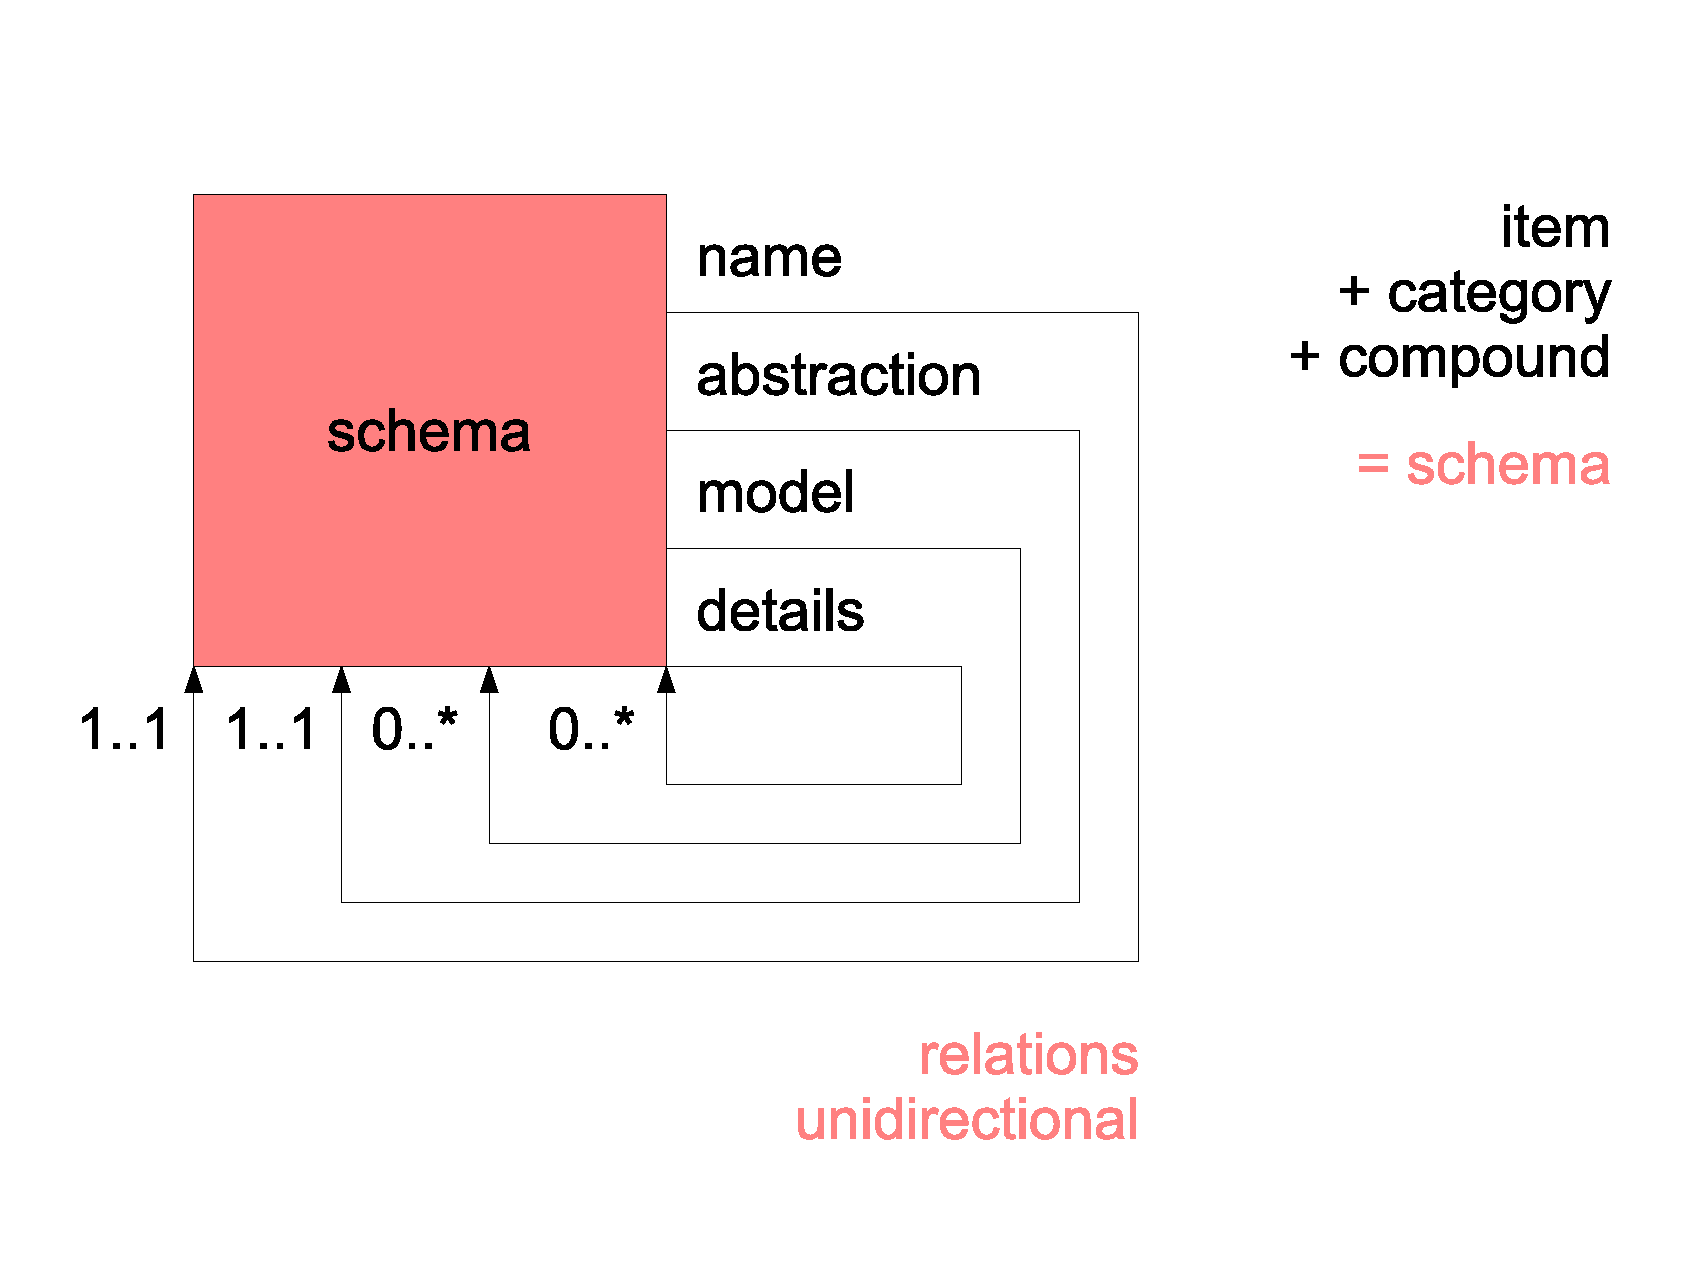
\includegraphics[scale=0.2]{vector/schema.eps}
        \caption{Knowledge Schema}
        \label{schema_figure}
    \end{center}
\end{figure}

Yet what does this knowledge of a compound model (whole) about its parts imply?
Software developers call knowledge \emph{about} something
\emph{Meta Information}. Figure \ref{schema_figure} illustrates a
\emph{Schema} (structure) with four kinds of meta information in a whole-part
relation.

An obvious way is to give each part a unique \emph{Name} for identification.
Secondly, a compound needs to know about the \emph{Model} of each part since a
part may itself be seen as compound that needs to know about its parts. The
distinction of the several kinds of models, in other words the kind of
\emph{Abstraction} (compound, term, number etc.) of a model is the third kind
of information a compound needs to know about its parts. It is comparable to a
\emph{Type} in classical system programming languages. All further kinds of
meta information are summed up by a fourth relation which is called
\emph{Details}.

%
% $RCSfile: double_hierarchy.tex,v $
%
% Copyright (C) 2002-2008. Christian Heller.
%
% Permission is granted to copy, distribute and/or modify this document
% under the terms of the GNU Free Documentation License, Version 1.1 or
% any later version published by the Free Software Foundation; with no
% Invariant Sections, with no Front-Cover Texts and with no Back-Cover
% Texts. A copy of the license is included in the section entitled
% "GNU Free Documentation License".
%
% http://www.cybop.net
% - Cybernetics Oriented Programming -
%
% http://www.resmedicinae.org
% - Information in Medicine -
%
% Version: $Revision: 1.1 $ $Date: 2008-08-19 20:41:06 $ $Author: christian $
% Authors: Christian Heller <christian.heller@tuxtax.de>
%

\subsection{Double Hierarchy}
\label{double_hierarchy_heading}
\index{Double Hierarchy}
\index{Whole-Part Relationship}
\index{Dialectical Relationship between Whole and Part}
\index{Conceptual Interaction}
\index{Part}
\index{Property}
\index{Constraint}

Finally, what makes up the character of a model (in the understanding of the
human mind) is a combination of two hierarchies: the \emph{Parts} it consists
of, together with \emph{Meta Information} about it.

Most properties of a molecule in \emph{Chemistry}, for example, are determined
by the number and arrangement of its atoms. \emph{Hydrogen} (H$_{2}$) becomes
\emph{Water} (H$_{2}$O) (with a totally different character) when just one
\emph{Oxygen} (O) atom is added per hydrogen molecule. The Wikipedia Encyclopedia
\cite{wikipedia} cites and writes about Richard Levins and Richard Lewontin
who, in their book \textit{The Dialectical Biologist} \cite{levins}, sketch a
\emph{dialectical} approach to biology:

\begin{quote}
    They focus on the (dialectical) relationship between the \emph{Whole} (or
    \emph{Totality}) and the \emph{Parts}: \textit{Part makes Whole, and Whole
    makes Part} \cite[p. 272]{levins}. That is, a biological system of some kind
    consists of a collection of heterogeneous parts. All of these contribute to
    the character of the whole, as in reductionist thinking. On the other hand,
    the whole has an existence independent of the parts and feeds back to affect
    and determine the nature of the parts. This back-and-forth (dialectic) of
    causation implies a dynamic process. \ldots\ Further, each species is part
    of the \emph{Environment} of all of the others.
\end{quote}

The kinds of meta information discussed in the previous sections were also
called \emph{Dimensions} or \emph{Conceptual Interaction} between a \emph{Whole}
and its \emph{Parts}. They may represent very different properties and each of
them may be constrained to certain values- or areas of validity.

\begin{figure}[ht]
    \begin{center}
        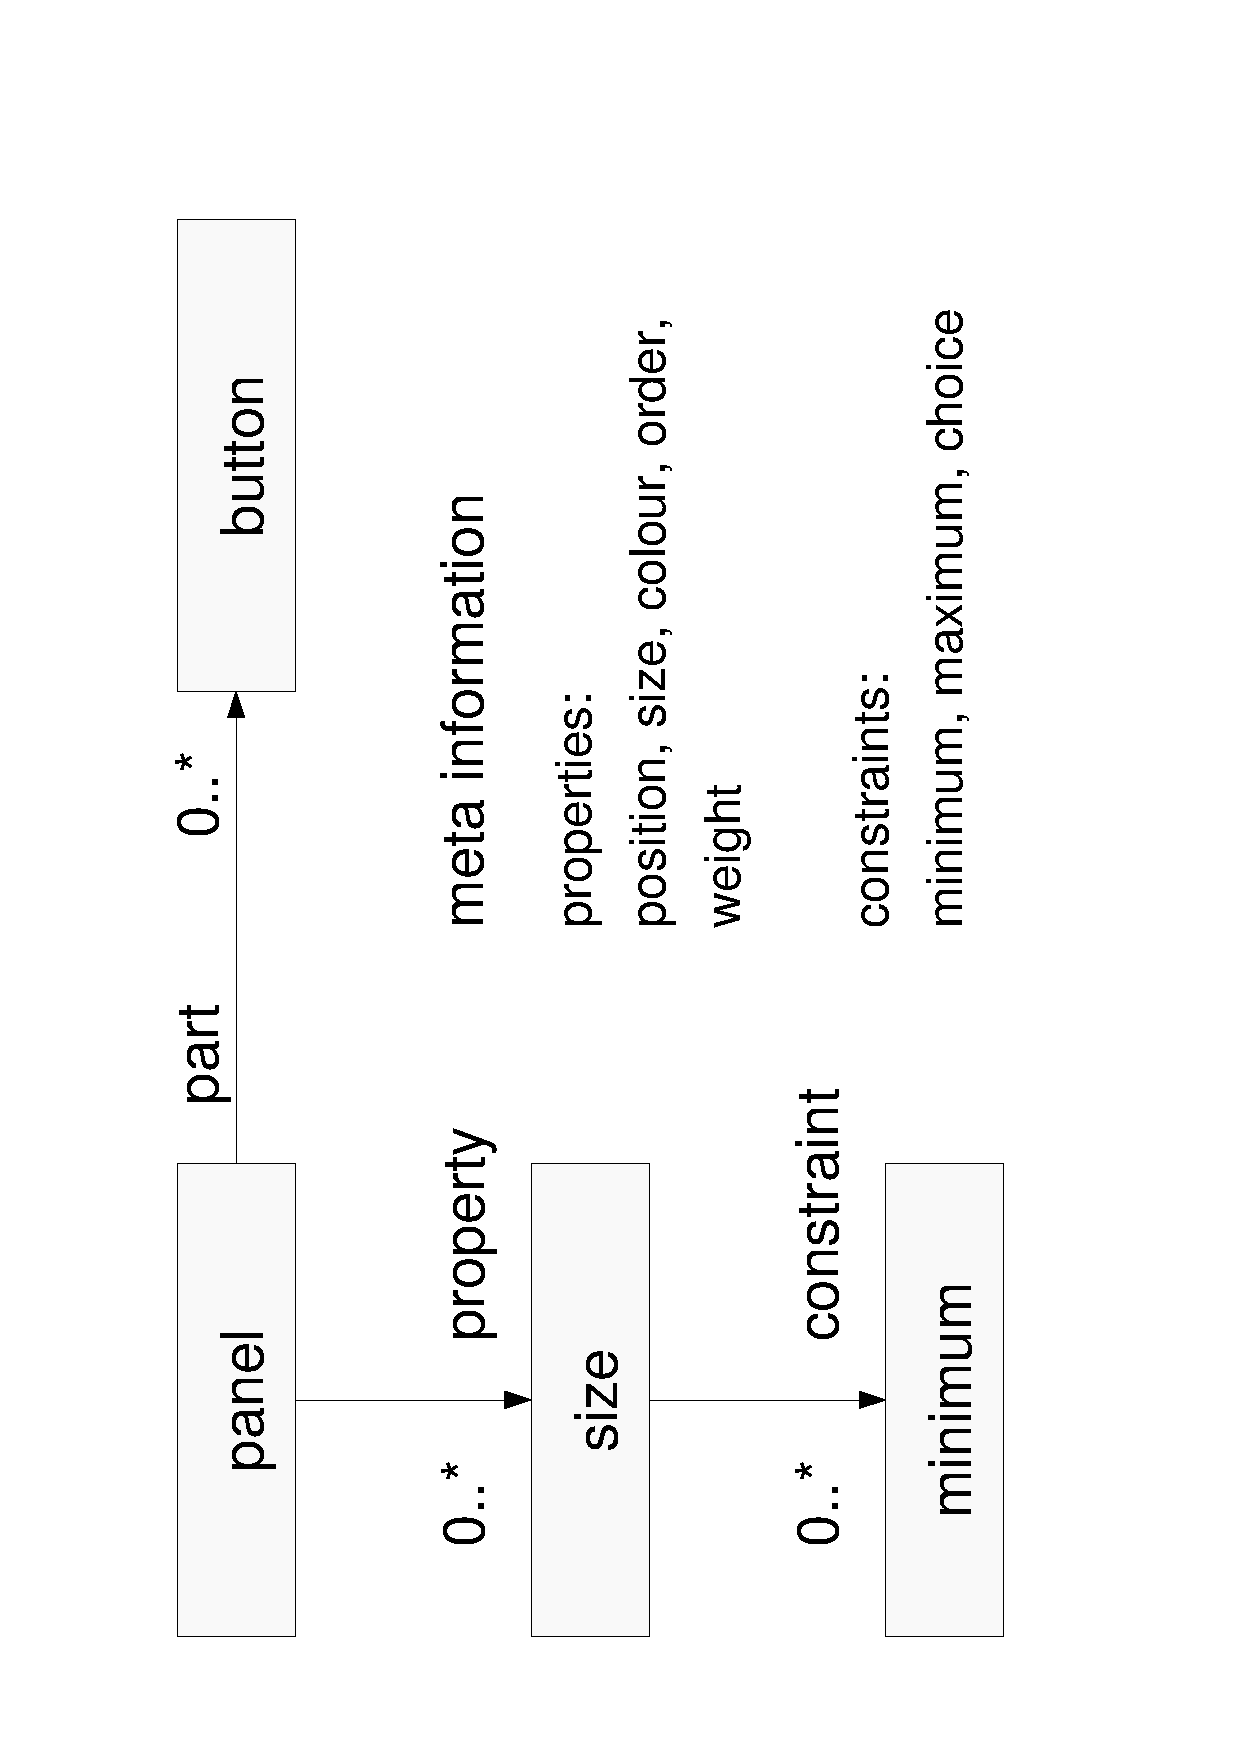
\includegraphics[scale=0.3,angle=-90]{graphic/double.pdf}
        \caption{Double Hierarchy of Parts and Meta Information}
        \label{double_figure}
    \end{center}
\end{figure}

Figure \ref{double_figure} illustrates the \emph{Double Hierarchy} here
spoken of. A graphical panel was chosen as example model. It may consist of
smaller parts, among them being a number of buttons. Altogether, they form the
\emph{Part Hierarchy}. On the other hand, there are properties like the size,
position or colour of the buttons, which are neither part of the panel, nor of
the buttons themselves; they are information \emph{about} the buttons and form
an own \emph{Meta Hierarchy}. To the latter do also belong constraints like the
minimum size of a button or a possible choice of colours for it. Constraints can
be treated like meta information about properties. Once again: \emph{Properties}
are information about a \emph{Part}; \emph{Constraints} are information about a
\emph{Property}.

%
% $RCSfile: modelling_example.tex,v $
%
% Copyright (C) 2002-2008. Christian Heller.
%
% Permission is granted to copy, distribute and/or modify this document
% under the terms of the GNU Free Documentation License, Version 1.1 or
% any later version published by the Free Software Foundation; with no
% Invariant Sections, with no Front-Cover Texts and with no Back-Cover
% Texts. A copy of the license is included in the section entitled
% "GNU Free Documentation License".
%
% http://www.cybop.net
% - Cybernetics Oriented Programming -
%
% http://www.resmedicinae.org
% - Information in Medicine -
%
% Version: $Revision: 1.1 $ $Date: 2008-08-19 20:41:07 $ $Author: christian $
% Authors: Christian Heller <christian.heller@tuxtax.de>
%

\subsection{Modelling Example}
\label{modelling_example_heading}
\index{Modelling Example}
\index{Concept of a Horse}
\index{Structured- and Procedural Programming}
\index{SPP}
\index{Object Oriented Programming}
\index{OOP}
\index{is-a Relation}
\index{has-a Relation}
\index{is-of Relation}
\index{Relation (is-a, has-a, is-of)}

Another example shall be given to substantiate the need to distinguish between
the several kinds of information. How would one describe a \emph{Horse},
unbiassed as a child, by doing some brainstorming? Figure \ref{horse_figure}
shows a number of terms commonly used to create a model of a horse. Most
importantly, there are structural observations describing the horse as concept
consisting of parts like \emph{Head}, \emph{Legs} or \emph{Hoofs}. Secondly,
there are properties like the horse's \emph{Colour}, \emph{Shape} or
\emph{Size}. Thirdly, there are terms describing a horse's actions like its
\emph{Movement} or \emph{Eating}, that change a horse's position and/ or state.
Finally, there are a number of terms like \emph{Hay} or \emph{Saddle}
associating concepts related to the horse.

\begin{figure}[ht]
    \begin{center}
        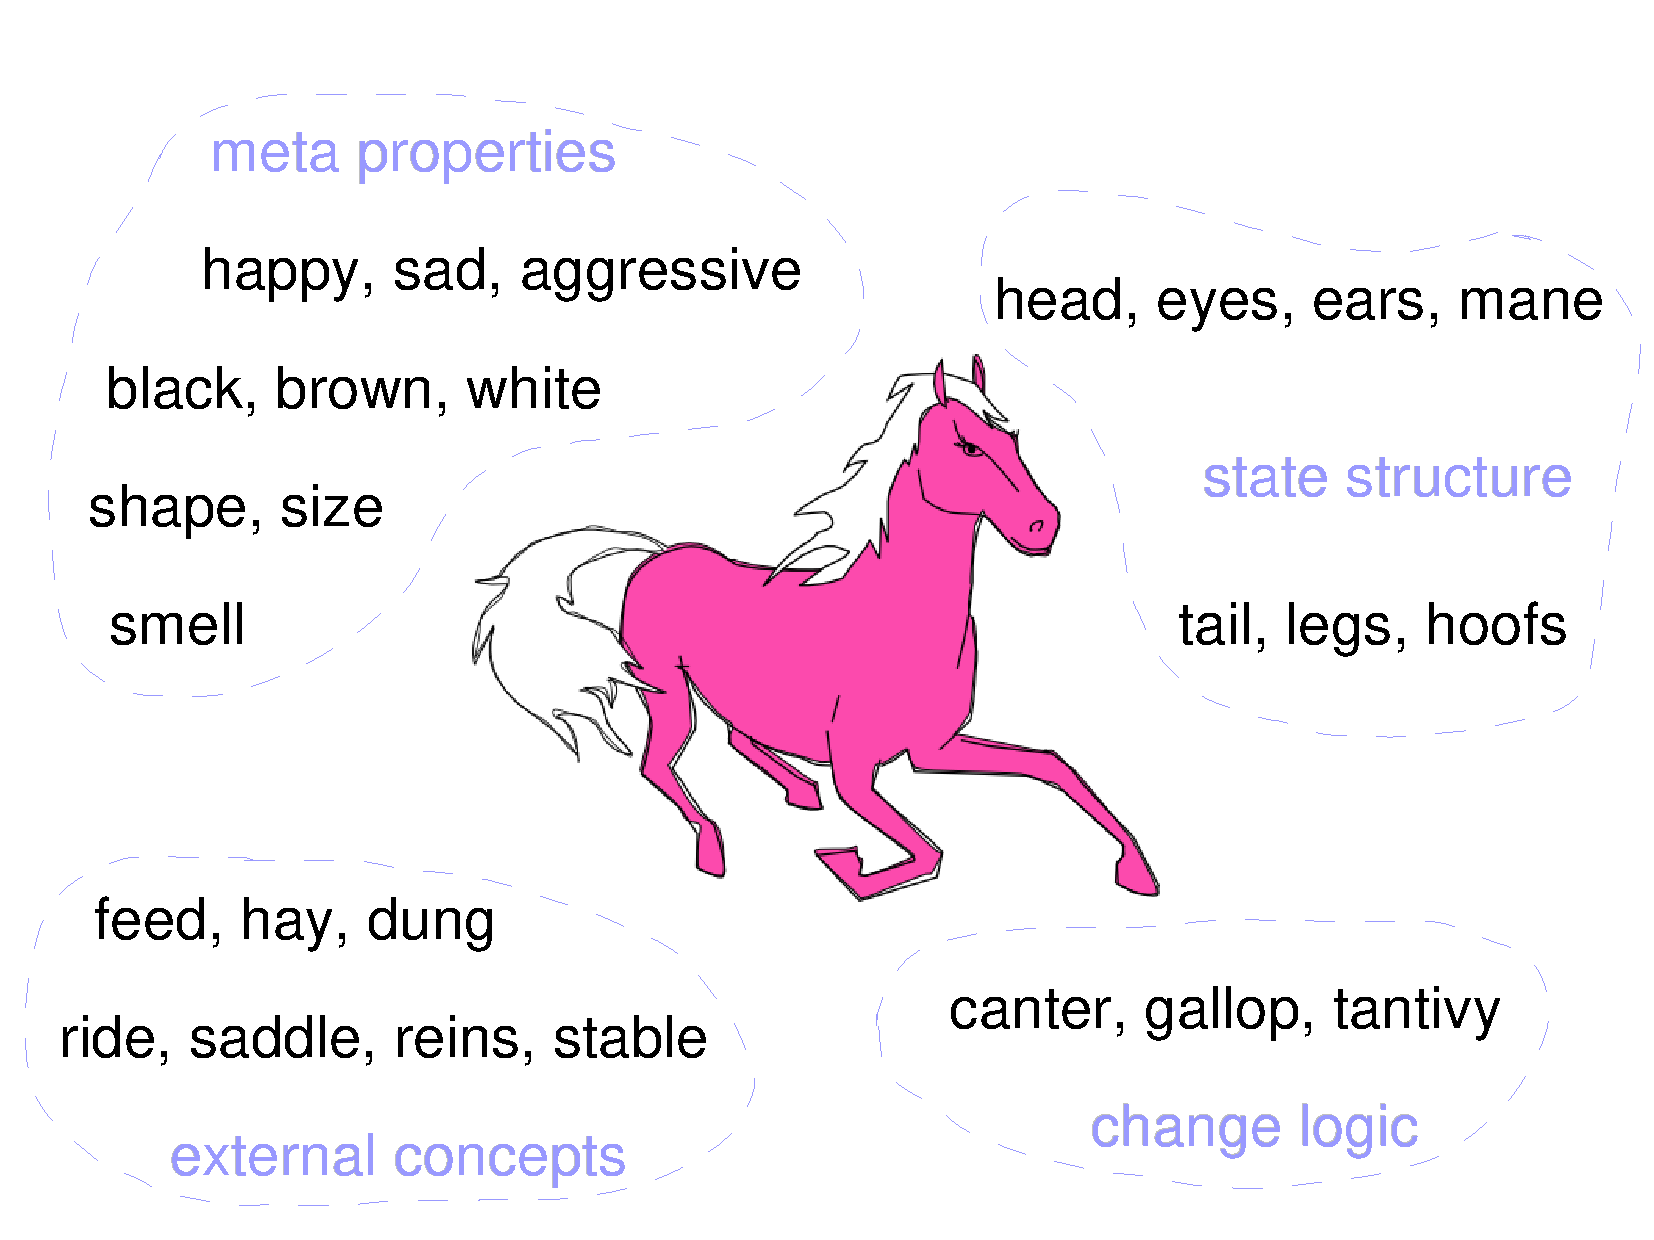
\includegraphics[scale=0.3,angle=-90]{graphic/horse.pdf}
        \caption{Concept of a Horse with Structure, Meta Properties and Logic}
        \label{horse_figure}
    \end{center}
\end{figure}

One might suggest to model properties like the position, size or colour of a
horse's leg as \emph{Part} of that leg. In fact, this is how classical
programming approaches its solutions.
\emph{Structured- and Procedural Programming} (SPP)
(section \ref{structured_and_procedural_programming_heading}), for example,
would probably use a structure called \emph{struct} or \emph{record}
representing the leg and a field standing for the leg's colour. Similarly,
\emph{Object Oriented Programming} (OOP)
(section \ref{object_oriented_programming_heading}) would use a class
representing the leg and an attribute standing for the leg's colour, which, in
Java source code, would look as follows:

\begin{scriptsize}
    \begin{verbatim}
    public class Leg {
        private String knee;
        private String hoof;
        private String colour;
    }
    \end{verbatim}
\end{scriptsize}

However, when following the modelling principles of human thinking (section
\ref{human_thinking_heading}), this is \emph{not} correct! It is true that in
everyday language, one tends to say \textit{A horse leg \emph{has a} colour.}
Unfortunately, this leads to the wrong assumption that a leg were made of a
colour. But this is not the case. A leg does not \emph{consist} of a colour in
the hierarchical meaning of a whole consisting of parts. The colour is rather
property information \emph{about} the leg. It seems there is no correct
expression in natural (English) language stating the property of something. The
\emph{IS-A} verbalisation is used to express that the leg belongs to a special
category of items, for example: \textit{A leg is a body element.} The
\emph{HAS-A} formulation is used to express that a leg as whole consists of
smaller parts, for example: \textit{A leg has a knee and it has a hoof.} But
which formulation expresses a property? Well, perhaps it would be best to say:
\textit{A leg IS-OF a colour.}

It seems that scientists (including the author of this work) and adults in
general have unlearnt to think simple like children. Scientists sometimes tend
to unnecessarily complicate things that can be described quite easy. Other
times, they simplify things which better be distinguished. And looking back
into the history of programming, one wonders who ever had this idea of mixing
structural elements, properties with meta information and logic algorithms into
just one structural entity as at least SPP (record, struct) and OOP (class) do.

The CYBOP knowledge schema introduced before takes care of these things and
distinguishes whole-part- from meta information. Actions (like the gallop of a
horse) causing some change in the model (horse) or its environment are called
\emph{Logic} in this work, since they follow certain rules. Chapter
\ref{state_and_logic_heading} will deal with these.

%
% $RCSfile$
%
% Copyright (c) 2002-2006. Christian Heller. All rights reserved.
%
% Permission is granted to copy, distribute and/or modify this document
% under the terms of the GNU Free Documentation License, Version 1.1 or
% any later version published by the Free Software Foundation; with no
% Invariant Sections, with no Front-Cover Texts and with no Back-Cover
% Texts. A copy of the license is included in the section entitled
% "GNU Free Documentation License".
%
% http://www.cybop.net
% - Cybernetics Oriented Programming -
%
% http://www.resmedicinae.org
% - Information in Medicine -
%
% Version: $Revision$ $Date$ $Author$
% Authors: Christian Heller <christian.heller@tuxtax.de>
%

\subsubsection{Container Unification}
\label{container_unification_heading}

Section \ref{motivation_heading} mentioned container inheritance as one problem
of current software. Due to polymorphism, it may cause unpredictable behaviour
possibly leading to \emph{falsified} container contents \cite{javaiaq}. The
previous sections introduced a knowledge schema which they claimed to be
\emph{general}. But that also means that all kinds of containers must be
representable by the suggested schema. But why are there so many different
kinds of containers? What actually is a container?

It is a concept expressing that some model \emph{contains} some other model(s).
Types of containers are, for example: \emph{Collections} (Array, Vector, Stack,
Set, List), \emph{Maps} (Hash Map, Hash Table) and the \emph{Tree}. They all
are containers. What differs, is just the meta information they store about
their elements. A list, for example, holds position information about each of
its elements. A map relates the name of an element to its model (1:1). A tree
links one model to many others (1:n).

But does the different meta information a container holds about its elements
justify the existence of different container models? If a knowledge schema was
general enough to represent a container structure on one hand, and to express
different kinds of meta information on the other, it might be able to behave
like any of the known container types.

The schema proposed in this work claims to be this kind of knowledge schema. It
has a container structure by default, and can thus hold many parts in a
\emph{Tree}-like manner. It holds standard meta information about its parts:
their \emph{Name}, \emph{Model}, kind of \emph{Abstraction} and further meta
information called \emph{Details} -- and is therefore able to link the name of
an element to its model, in a \emph{Map}-like manner. To the additional meta
information (details) may belong the \emph{Position} of an element within its
model, in a \emph{List}-like manner. A \emph{Table} structure can be represented
as well, by splitting it into a hierarchical (tree-like) representation, as
known from markup languages like the \emph{Hypertext Markup Language} (HTML).

Section \ref{cybol_heading} will introduce a language capable of expressing all
aspects of the knowledge schema as proposed here.

%
% $RCSfile: universal_memory_structure.tex,v $
%
% Copyright (C) 2002-2008. Christian Heller.
%
% Permission is granted to copy, distribute and/or modify this document
% under the terms of the GNU Free Documentation License, Version 1.1 or
% any later version published by the Free Software Foundation; with no
% Invariant Sections, with no Front-Cover Texts and with no Back-Cover
% Texts. A copy of the license is included in the section entitled
% "GNU Free Documentation License".
%
% http://www.cybop.net
% - Cybernetics Oriented Programming -
%
% http://www.resmedicinae.org
% - Information in Medicine -
%
% Version: $Revision: 1.1 $ $Date: 2008-08-19 20:41:09 $ $Author: christian $
% Authors: Christian Heller <christian.heller@tuxtax.de>
%

\subsection{Universal Memory Structure}
\label{universal_memory_structure_heading}
\index{Universal Memory Structure}
\index{Structured- and Procedural Programming}
\index{SPP}
\index{Object Oriented Programming}
\index{OOP}
\index{Design Time Structure}
\index{Runtime Structure}
\index{Knowledge Schema}

To better explain the differences between traditional- and cybernetics-oriented
design models, a further example shall be given. Figure \ref{universal_figure}
illustrates design-time structures in the upper half, and runtime structures in
the lower. Using \emph{Structured- and Procedural Programming} (SPP) or
\emph{Object Oriented Programming} (OOP), a developer would design a model as
shown on the upper left-hand side in the figure. (The fact that OOP also offers
inheritance relations and OOP classes do own methods in addition to attributes,
while SPP structures do not, is of minor importance here.) At runtime, exactly
that model would be applied to structure instances and their relations
accordingly, as shown on the lower left-hand side in the figure.

\begin{figure}[ht]
    \begin{center}
        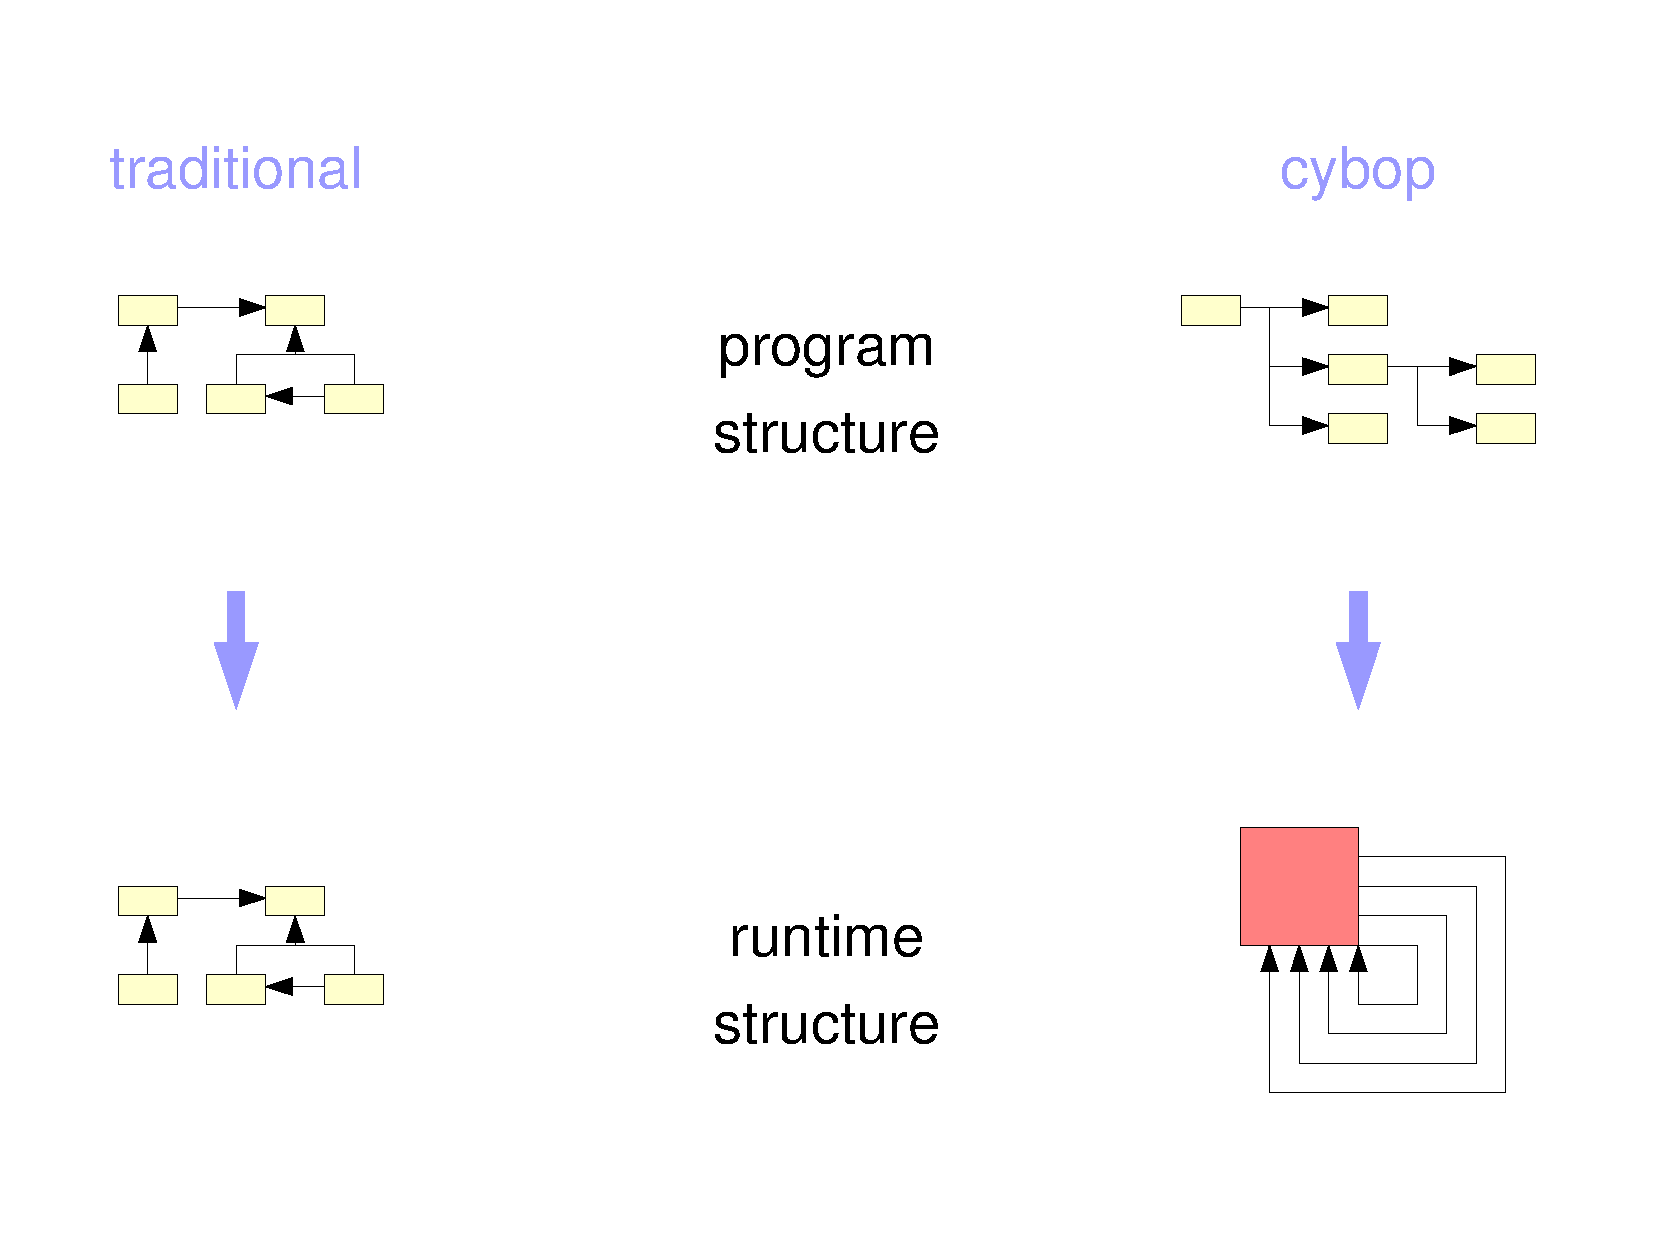
\includegraphics[scale=0.3,angle=-90]{graphic/universal.pdf}
        \caption{Universal Memory Structure}
        \label{universal_figure}
    \end{center}
\end{figure}

Not so in \emph{Cybernetics Oriented Programming} (CYBOP). Knowledge templates
as created at design time do always have a hierarchical structure, as shown on
the upper right-hand side in the figure. They include \emph{Whole-Part-} as
well as \emph{Meta Hierarchies}. At runtime, these templates get cloned by
creating models that follow the structure of the CYBOP \emph{Knowledge Schema},
as shown on the lower right-hand side in the figure. While SPP/ OOP rely on a
variety of different structures to store knowledge in memory, CYBOP uses one
\emph{Universal Memory Structure} (knowledge schema) that, so to say, merges
traditional structures like different kinds of \emph{Containers}, \emph{Class}
and \emph{Record}/\emph{Struct}. Even algorithmic structures (logic)
traditionally stored in a \emph{Procedure} are covered by this knowledge
schema. More on state and logic in the following chapter.

The advantages are obvious. Data available in a unified structure are easier to
process. Dependencies of the knowledge schema are defined clearly and remain
the same for all applications, so that domain/ application knowledge becomes
independent from the underlying system control software. Global data access and
bidirectional dependencies are not necessary anymore, since every knowledge
model can be accessed along well-defined paths within the knowledge hierarchy.
Byte code manipulation and similar tricks and workarounds might finally belong
to the past.


